\KOMAoption{paper}{a4, portrait}
\areaset{267mm}{180mm}
\fancyheadoffset{0pt} % обновляем хедер и футер

\newgeometry{
  top=14mm,
  bottom=11mm,
  right=10mm,
  left=22mm,
}

\begin{landscape}

%\setlength{\headsep}{5.6mm} 
%\setlength{\topmargin}{-27mm}
\setlength{\footskip}{15.5pt}
%\setlength{\textwidth}{305mm}

\color{uniblue}{\section[(справочное) Перечень сигналов ФСУ, предназначенных \newline для конфигурирования устройства <<ЮНИТ-М300-ОЛ>>]{(справочное)\\Перечень сигналов ФСУ, предназначенных для конфигурирования устройства <<ЮНИТ-М300-ОЛ>>}\label{app:signals}}
\color{black}

\begin{enumerate}[label=\ref{app:signals}.\arabic*] % Без глобального влияния
  \item Перечень сигналов самодиагностики, доступных для конфигурирования, приведен в документации ЮТКБ.656122.609 РЭ <<Устройство защиты и автоматики серии <<ЮНИТ-М300>>. Руководство по эксплуатации общее>>.
  \item Условные обозначения, применяемые в таблице перечня сигналов:
  \begin{itemize}
    \item[$\text{(--)}$] { - сигнал не имеет возможности конфигурации;}
    \item[$\text{(+)}$] { - сигнал имеет возможность конфигурации;}
    \item[$\text{(*)}$] { - конфигурация сигнала предустановлена по умолчанию в сервисном ПО <<ЮНИТ-СЕРВИС>> и не может быть изменена.}
  \end{itemize}
\end{enumerate}

\small % сделаем шрифт в таблице поменьше
% В таблице ниже убрал правую и левую горизонтальные линии чтобы не сливались и жирно видно - также в настройках geometry прищлось поле right =8mm а не 5 mm 
% так как строки ниже колонтитулов спускались
\begin{longtable}{
>{\centering\arraybackslash}m{6.0cm}
|>{\centering\arraybackslash}m{3.45cm}
|>{\centering\arraybackslash}m{2cm}
|>{\centering\arraybackslash}m{2cm}
|>{\centering\arraybackslash}m{2cm}
|>{\centering\arraybackslash}m{2cm}
|>{\centering\arraybackslash}m{2cm}
|>{\centering\arraybackslash}m{2cm}
|>{\centering\arraybackslash}m{2.107cm}
}

%\caption{Перечень сигналов ФСУ, предназначенных для конфигурирования устройств ЮНИТ-М300\vspace{-0.5\baselineskip}}\label{appA:tbl1}\\ % выравнивает надпись посередине таблицы
\caption{Перечень сигналов ФСУ, предназначенных для конфигурирования устройства\hfill\vspace{-0.5\baselineskip}}\label{appA:tbl1}\\ 

\hline
\rowcolor{gray!30}
Полное наименование сигнала & Наименование сигнала на ФСУ & Дискретные входы & Выходные реле & Светодиоды & Функционал. клавиши & Регистратор событий & Аварийный осциллограф & Пуск авар. осциллографа \\ 
\hline
\endfirsthead
%\caption{\emph{Продолжение\vspace{-0.5\baselineskip}}} \\ % Отступ обозначения таблицы от таблицы и выравнивание надписи слева
\caption*{\hspace{3pt}\emph{Продолжение таблицы \ref{appA:tbl1}\hfill\vspace{-0.5\baselineskip}}} \\ % сделано по ГОСТ 2.105 п.6.8.7
\hline
\rowcolor{gray!30}
Полное наименование сигнала & Наименование сигнала на ФСУ & Дискретные входы & Выходные реле & Светодиоды & Функционал. клавиши & Регистратор событий & Аварийный осциллограф & Пуск авар. осциллографа \\ 
%\hline
\endhead

%\hline
\endfoot

%\hline
\endlastfoot

%===t2
\multicolumn{9}{c}{\textbf{Виртуальные кнопки}} \\
\hline
\raggedright Сброс & \centering Сброс & \centering -- & \centering -- & \centering -- & \centering + & \centering + & \centering + & \centering \arraybackslash + \\ \hline
\raggedright Сброс счетчика операций В & \centering Сброс счет.опер.В & \centering -- & \centering -- & \centering -- & \centering + & \centering + & \centering + & \centering \arraybackslash + \\ \hline
\raggedright Сброс счетчика операций ВЭ & \centering Сброс счет.опер.ВЭ & \centering -- & \centering -- & \centering -- & \centering + & \centering + & \centering + & \centering \arraybackslash + \\ \hline
\raggedright Сброс счетчика операций ЗН & \centering Сброс счет.опер.ЗН & \centering -- & \centering -- & \centering -- & \centering + & \centering + & \centering + & \centering \arraybackslash + \\ \hline
\raggedright Сброс счетчиков ресурса выключателя & \centering Сброс КРВ & \centering -- & \centering -- & \centering -- & \centering + & \centering + & \centering + & \centering \arraybackslash + \\ \hline
\multicolumn{9}{c}{\textbf{Виртуальные ключи}} \\
\hline
\raggedright Вывод терминала & \centering Вывод терминала & \centering -- & \centering -- & \centering -- & \centering + & \centering + & \centering + & \centering \arraybackslash + \\ \hline
\raggedright Оперативный вывод функции ДЗ & \centering ОВ ДЗ & \centering -- & \centering -- & \centering -- & \centering + & \centering + & \centering + & \centering \arraybackslash + \\ \hline
\raggedright Оперативный вывод 1 ступени ДЗ-фф & \centering ОВ ДЗ-фф 1ст. & \centering -- & \centering -- & \centering -- & \centering + & \centering + & \centering + & \centering \arraybackslash + \\ \hline
\raggedright Перевод 1 ступени ДЗ-фф на сигнал & \centering ДЗ-фф 1ст. на сигн & \centering -- & \centering -- & \centering -- & \centering + & \centering + & \centering + & \centering \arraybackslash + \\ \hline
\raggedright Оперативный вывод 2 ступени ДЗ-фф & \centering ОВ ДЗ-фф 2ст. & \centering -- & \centering -- & \centering -- & \centering + & \centering + & \centering + & \centering \arraybackslash + \\ \hline
\raggedright Перевод 2 ступени ДЗ-фф на сигнал & \centering ДЗ-фф 2ст. на сигн & \centering -- & \centering -- & \centering -- & \centering + & \centering + & \centering + & \centering \arraybackslash + \\ \hline
\raggedright Оперативный вывод 3 ступени ДЗ-фф & \centering ОВ ДЗ-фф 3ст. & \centering -- & \centering -- & \centering -- & \centering + & \centering + & \centering + & \centering \arraybackslash + \\ \hline
\raggedright Перевод 3 ступени ДЗ-фф на сигнал & \centering ДЗ-фф 3ст. на сигн & \centering -- & \centering -- & \centering -- & \centering + & \centering + & \centering + & \centering \arraybackslash + \\ \hline
\raggedright Оперативный вывод 1 ступени ДЗ-фз & \centering ОВ ДЗ-фз 1ст. & \centering -- & \centering -- & \centering -- & \centering + & \centering + & \centering + & \centering \arraybackslash + \\ \hline
\raggedright Перевод 1 ступени ДЗ-фз на сигнал & \centering ДЗ-фз 1ст. на сигн & \centering -- & \centering -- & \centering -- & \centering + & \centering + & \centering + & \centering \arraybackslash + \\ \hline
\raggedright Оперативный вывод 2 ступени ДЗ-фз & \centering ОВ ДЗ-фз 2ст. & \centering -- & \centering -- & \centering -- & \centering + & \centering + & \centering + & \centering \arraybackslash + \\ \hline
\raggedright Перевод 2 ступени ДЗ-фз на сигнал & \centering ДЗ-фз 2ст. на сигн & \centering -- & \centering -- & \centering -- & \centering + & \centering + & \centering + & \centering \arraybackslash + \\ \hline
\raggedright Сигнал ввода оперативного ускорения ДЗ & \centering Ввод ОУ ДЗ & \centering -- & \centering -- & \centering -- & \centering + & \centering + & \centering + & \centering \arraybackslash + \\ \hline
\raggedright Оперативный вывод функции БК & \centering ОВ БК & \centering -- & \centering -- & \centering -- & \centering + & \centering + & \centering + & \centering \arraybackslash + \\ \hline
\raggedright Оперативный вывод функции ТО & \centering ОВ ТО & \centering -- & \centering -- & \centering -- & \centering + & \centering + & \centering + & \centering \arraybackslash + \\ \hline
\raggedright Перевод ТО на сигнал & \centering ТО на сигн & \centering -- & \centering -- & \centering -- & \centering + & \centering + & \centering + & \centering \arraybackslash + \\ \hline
\raggedright Оперативный вывод функции МТЗ & \centering ОВ МТЗ & \centering -- & \centering -- & \centering -- & \centering + & \centering + & \centering + & \centering \arraybackslash + \\ \hline
\raggedright Оперативный вывод 1 ступени МТЗ & \centering ОВ МТЗ 1 ст. & \centering -- & \centering -- & \centering -- & \centering + & \centering + & \centering + & \centering \arraybackslash + \\ \hline
\raggedright Перевод МТЗ 1 ступени на сигнал & \centering МТЗ 1ст. на сигн & \centering -- & \centering -- & \centering -- & \centering + & \centering + & \centering + & \centering \arraybackslash + \\ \hline
\raggedright Оперативный вывод 2 ступени МТЗ & \centering ОВ МТЗ 2 ст. & \centering -- & \centering -- & \centering -- & \centering + & \centering + & \centering + & \centering \arraybackslash + \\ \hline
\raggedright Перевод МТЗ 2 ступени на сигнал & \centering МТЗ 2ст. на сигн & \centering -- & \centering -- & \centering -- & \centering + & \centering + & \centering + & \centering \arraybackslash + \\ \hline
\raggedright Оперативный вывод 3 ступени МТЗ & \centering ОВ МТЗ 3 ст. & \centering -- & \centering -- & \centering -- & \centering + & \centering + & \centering + & \centering \arraybackslash + \\ \hline
\raggedright Перевод МТЗ 3 ступени на сигнал & \centering МТЗ 3ст. на сигн & \centering -- & \centering -- & \centering -- & \centering + & \centering + & \centering + & \centering \arraybackslash + \\ \hline
\raggedright Сигнал ввода оперативного ускорения МТЗ & \centering Ввод ОУ МТЗ & \centering -- & \centering -- & \centering -- & \centering + & \centering + & \centering + & \centering \arraybackslash + \\ \hline
\raggedright Оперативный вывод функции АУ & \centering ОВ АУ & \centering -- & \centering -- & \centering -- & \centering + & \centering + & \centering + & \centering \arraybackslash + \\ \hline
\raggedright Оперативный вывод функции ТЗНП & \centering ОВ ТЗНП & \centering -- & \centering -- & \centering -- & \centering + & \centering + & \centering + & \centering \arraybackslash + \\ \hline
\raggedright Перевод ТЗНП 1 ступени на сигнал & \centering ТЗНП 1ст. на сигн & \centering -- & \centering -- & \centering -- & \centering + & \centering + & \centering + & \centering \arraybackslash + \\ \hline
\raggedright Режим работы ЧС & \centering Режим работы ЧС & \centering -- & \centering -- & \centering -- & \centering + & \centering + & \centering + & \centering \arraybackslash + \\ \hline
\raggedright Перевод ТЗНП 2 ступени на сигнал & \centering ТЗНП 2ст. на сигн & \centering -- & \centering -- & \centering -- & \centering + & \centering + & \centering + & \centering \arraybackslash + \\ \hline
\raggedright Сигнал ввода оперативного ускорения ТЗНП & \centering Ввод ОУ ТЗНП & \centering -- & \centering -- & \centering -- & \centering + & \centering + & \centering + & \centering \arraybackslash + \\ \hline
\raggedright Оперативный вывод функции НЗОЗЗ & \centering ОВ НЗОЗЗ & \centering -- & \centering -- & \centering -- & \centering + & \centering + & \centering + & \centering \arraybackslash + \\ \hline
\raggedright Перевод НЗОЗЗ на сигнал & \centering НЗОЗЗ на сигн & \centering -- & \centering -- & \centering -- & \centering + & \centering + & \centering + & \centering \arraybackslash + \\ \hline
\raggedright Оперативный вывод функции ЗДЗ & \centering ОВ ЗДЗ & \centering -- & \centering -- & \centering -- & \centering + & \centering + & \centering + & \centering \arraybackslash + \\ \hline
\raggedright Перевод ЗДЗ на сигнал & \centering ЗДЗ на сигн & \centering -- & \centering -- & \centering -- & \centering + & \centering + & \centering + & \centering \arraybackslash + \\ \hline
\raggedright Оперативный вывод функции ЗОП & \centering ОВ ЗОП & \centering -- & \centering -- & \centering -- & \centering + & \centering + & \centering + & \centering \arraybackslash + \\ \hline
\raggedright Перевод ЗОП на сигнал & \centering ЗОП на сигн & \centering -- & \centering -- & \centering -- & \centering + & \centering + & \centering + & \centering \arraybackslash + \\ \hline
\raggedright Оперативный вывод функции ЗП & \centering ОВ ЗП & \centering -- & \centering -- & \centering -- & \centering + & \centering + & \centering + & \centering \arraybackslash + \\ \hline
\raggedright Перевод ЗП на отключение & \centering ЗП на откл & \centering -- & \centering -- & \centering -- & \centering + & \centering + & \centering + & \centering \arraybackslash + \\ \hline
\raggedright Оперативный вывод функции ГСОЗЗ & \centering ОВ ГСОЗЗ & \centering -- & \centering -- & \centering -- & \centering + & \centering + & \centering + & \centering \arraybackslash + \\ \hline
\raggedright Перевод ГСОЗЗ на отключение & \centering ГСОЗЗ на откл & \centering -- & \centering -- & \centering -- & \centering + & \centering + & \centering + & \centering \arraybackslash + \\ \hline
\raggedright Оперативный вывод функции ГЗсигн & \centering ОВ ЛО ГЗсигн & \centering -- & \centering -- & \centering -- & \centering + & \centering + & \centering + & \centering \arraybackslash + \\ \hline
\raggedright Перевод ГЗсигн на отключение & \centering ЛО ГЗсигн на откл & \centering -- & \centering -- & \centering -- & \centering + & \centering + & \centering + & \centering \arraybackslash + \\ \hline
\raggedright Оперативный вывод функции ГЗоткл & \centering ОВ ЛО ГЗоткл & \centering -- & \centering -- & \centering -- & \centering + & \centering + & \centering + & \centering \arraybackslash + \\ \hline
\raggedright Перевод ГЗоткл на сигнал & \centering ЛО ГЗоткл на сигн & \centering -- & \centering -- & \centering -- & \centering + & \centering + & \centering + & \centering \arraybackslash + \\ \hline
\raggedright Оперативный вывод функции ЛО ТЗ & \centering ОВ ЛО ТЗ & \centering -- & \centering -- & \centering -- & \centering + & \centering + & \centering + & \centering \arraybackslash + \\ \hline
\raggedright Оперативный вывод ЛО ДТм & \centering ОВ ЛО ДТм & \centering -- & \centering -- & \centering -- & \centering + & \centering + & \centering + & \centering \arraybackslash + \\ \hline
\raggedright Перевод ДТм на сигнал & \centering ЛО ДТм на сигн & \centering -- & \centering -- & \centering -- & \centering + & \centering + & \centering + & \centering \arraybackslash + \\ \hline
\raggedright Оперативный вывод ЛО ДТо & \centering ОВ ЛО ДТо & \centering -- & \centering -- & \centering -- & \centering + & \centering + & \centering + & \centering \arraybackslash + \\ \hline
\raggedright Перевод ДТо на сигнал & \centering ЛО ДТо на сигн & \centering -- & \centering -- & \centering -- & \centering + & \centering + & \centering + & \centering \arraybackslash + \\ \hline
\raggedright Оперативный вывод ЛО РД & \centering ОВ ЛО РД & \centering -- & \centering -- & \centering -- & \centering + & \centering + & \centering + & \centering \arraybackslash + \\ \hline
\raggedright Перевод РД на сигнал & \centering ЛО РД на сигн & \centering -- & \centering -- & \centering -- & \centering + & \centering + & \centering + & \centering \arraybackslash + \\ \hline
\raggedright Оперативный вывод функции УРОВ & \centering ОВ УРОВ & \centering -- & \centering -- & \centering -- & \centering + & \centering + & \centering + & \centering \arraybackslash + \\ \hline
\raggedright Оперативный вывод функции ЗМН & \centering ОВ ЗМН & \centering -- & \centering -- & \centering -- & \centering + & \centering + & \centering + & \centering \arraybackslash + \\ \hline
\raggedright Перевод ЗМН на сигнал & \centering ЗМН на сигн & \centering -- & \centering -- & \centering -- & \centering + & \centering + & \centering + & \centering \arraybackslash + \\ \hline
\raggedright Оперативный вывод функции ЗПН & \centering ОВ ЗПН & \centering -- & \centering -- & \centering -- & \centering + & \centering + & \centering + & \centering \arraybackslash + \\ \hline
\raggedright Перевод ЗПН на сигнал & \centering ЗПН на сигн & \centering -- & \centering -- & \centering -- & \centering + & \centering + & \centering + & \centering \arraybackslash + \\ \hline
\raggedright Оперативный вывод функции БННш & \centering ОВ БННш & \centering -- & \centering -- & \centering -- & \centering + & \centering + & \centering + & \centering \arraybackslash + \\ \hline
\raggedright Фиксация неисправности цепей напряжения шин & \centering Фикс.неисп.ЦНш & \centering -- & \centering -- & \centering -- & \centering + & \centering + & \centering + & \centering \arraybackslash + \\ \hline
\raggedright Оперативный вывод функции БННп & \centering ОВ БННп & \centering -- & \centering -- & \centering -- & \centering + & \centering + & \centering + & \centering \arraybackslash + \\ \hline
\raggedright Оперативный вывод функции ЗСЧ & \centering ОВ ЗСЧ & \centering -- & \centering -- & \centering -- & \centering + & \centering + & \centering + & \centering \arraybackslash + \\ \hline
\raggedright Перевод ЗСЧ на сигнал & \centering ЗСЧ на сигн & \centering -- & \centering -- & \centering -- & \centering + & \centering + & \centering + & \centering \arraybackslash + \\ \hline
\raggedright Оперативный вывод функции ЗПЧ & \centering ОВ ЗПЧ & \centering -- & \centering -- & \centering -- & \centering + & \centering + & \centering + & \centering \arraybackslash + \\ \hline
\raggedright Перевод ЗПЧ на сигнал & \centering ЗПЧ на сигн & \centering -- & \centering -- & \centering -- & \centering + & \centering + & \centering + & \centering \arraybackslash + \\ \hline
\raggedright Оперативный вывод функции ЗИЧ & \centering ОВ ЗИЧ & \centering -- & \centering -- & \centering -- & \centering + & \centering + & \centering + & \centering \arraybackslash + \\ \hline
\raggedright Перевод ЗИЧ на сигнал & \centering ЗИЧ на сигн & \centering -- & \centering -- & \centering -- & \centering + & \centering + & \centering + & \centering \arraybackslash + \\ \hline
\raggedright Оперативный вывод функции АЧР & \centering ОВ АЧР & \centering -- & \centering -- & \centering -- & \centering + & \centering + & \centering + & \centering \arraybackslash + \\ \hline
\raggedright Оперативный вывод функции ЧАПВ & \centering ОВ ЧАПВ & \centering -- & \centering -- & \centering -- & \centering + & \centering + & \centering + & \centering \arraybackslash + \\ \hline
\raggedright Оперативный вывод функции АПВ & \centering ОВ АПВ & \centering -- & \centering -- & \centering -- & \centering + & \centering + & \centering + & \centering \arraybackslash + \\ \hline
\raggedright Блокировка второго цикла & \centering АПВ Блок. 2 цикла & \centering -- & \centering -- & \centering -- & \centering + & \centering + & \centering + & \centering \arraybackslash + \\ \hline
\raggedright АПВ без контролей & \centering АПВ Без контролей & \centering -- & \centering -- & \centering -- & \centering + & \centering + & \centering + & \centering \arraybackslash + \\ \hline
\raggedright АПВ с контролем от КННш и КОНп & \centering АПВ КННш+КОНп & \centering -- & \centering -- & \centering -- & \centering + & \centering + & \centering + & \centering \arraybackslash + \\ \hline
\raggedright АПВ с контролем от КОНш и КННп & \centering АПВ КОНш+КННп & \centering -- & \centering -- & \centering -- & \centering + & \centering + & \centering + & \centering \arraybackslash + \\ \hline
\raggedright Оперативный вывод функции КННш & \centering ОВ КННш & \centering -- & \centering -- & \centering -- & \centering + & \centering + & \centering + & \centering \arraybackslash + \\ \hline
\raggedright Оперативный вывод функции КННп & \centering ОВ КННп & \centering -- & \centering -- & \centering -- & \centering + & \centering + & \centering + & \centering \arraybackslash + \\ \hline
\raggedright Оперативный вывод функции КОНш & \centering ОВ КОНш & \centering -- & \centering -- & \centering -- & \centering + & \centering + & \centering + & \centering \arraybackslash + \\ \hline
\raggedright Оперативный вывод функции КОНп & \centering ОВ КОНп & \centering -- & \centering -- & \centering -- & \centering + & \centering + & \centering + & \centering \arraybackslash + \\ \hline
\raggedright Оперативный вывод функции КС & \centering ОВ КС & \centering -- & \centering -- & \centering -- & \centering + & \centering + & \centering + & \centering \arraybackslash + \\ \hline
\raggedright Оперативный вывод функции ЛОВ & \centering ОВ ЛОВ & \centering -- & \centering -- & \centering -- & \centering + & \centering + & \centering + & \centering \arraybackslash + \\ \hline
\raggedright Оперативный вывод ЛО РЗ & \centering ОВ ЛО РЗ & \centering -- & \centering -- & \centering -- & \centering + & \centering + & \centering + & \centering \arraybackslash + \\ \hline
\raggedright Оперативный вывод ПА & \centering ОВ ПА & \centering -- & \centering -- & \centering -- & \centering + & \centering + & \centering + & \centering \arraybackslash + \\ \hline
\raggedright Оперативный вывод функции КП & \centering ОВ КП & \centering -- & \centering -- & \centering -- & \centering + & \centering + & \centering + & \centering \arraybackslash + \\ \hline
\raggedright Программная деблокировка управления выкатным элементом & \centering Програм. деблок. ВЭ & \centering -- & \centering -- & \centering -- & \centering + & \centering + & \centering + & \centering \arraybackslash + \\ \hline
\raggedright Программная деблокировка управления заземляющим ножом & \centering Програм. деблок. ЗН & \centering -- & \centering -- & \centering -- & \centering + & \centering + & \centering + & \centering \arraybackslash + \\ \hline
\raggedright Оперативный вывод функции УВ & \centering ОВ УВ & \centering -- & \centering -- & \centering -- & \centering + & \centering + & \centering + & \centering \arraybackslash + \\ \hline
\raggedright Оперативный вывод функции КА & \centering ОВ КА & \centering -- & \centering -- & \centering -- & \centering + & \centering + & \centering + & \centering \arraybackslash + \\ \hline
\raggedright Оперативный вывод функции КСВ & \centering ОВ КСВ & \centering -- & \centering -- & \centering -- & \centering + & \centering + & \centering + & \centering \arraybackslash + \\ \hline
\raggedright Оперативный вывод функции ПДС & \centering ОВ ПДС & \centering -- & \centering -- & \centering -- & \centering + & \centering + & \centering + & \centering \arraybackslash + \\ \hline
\raggedright Оперативный вывод функции ПДС НКУ & \centering ОВ ПДС НКУ & \centering -- & \centering -- & \centering -- & \centering + & \centering + & \centering + & \centering \arraybackslash + \\ \hline
\multicolumn{9}{c}{\textbf{Общие сигналы функциональной логики}} \\
\hline
\rowcolor{gray!15} 
\multicolumn{9}{c}{Дистанционная защита (ДЗ)} \\
\hline
\multicolumn{9}{c}{1 ступень дистанционной защиты по контуру «фаза-фаза» (ДЗ-фф 1ст.)} \\
\hline
\raggedright Функция введена в работу & \centering Ввод & \centering -- & \centering + & \centering + & \centering -- & \centering + & \centering + & \centering \arraybackslash + \\ \hline
\raggedright Функция оперативно выведена из работы & \centering Оперативный вывод & \centering -- & \centering + & \centering + & \centering -- & \centering + & \centering + & \centering \arraybackslash + \\ \hline
\raggedright Пуск ИО сопротивления Zab (фаза-фаза1) & \centering ИО Zab & \centering -- & \centering + & \centering + & \centering -- & \centering + & \centering + & \centering \arraybackslash + \\ \hline
\raggedright Пуск ИО сопротивления Zbc (фаза-фаза1) & \centering ИО Zbc & \centering -- & \centering + & \centering + & \centering -- & \centering + & \centering + & \centering \arraybackslash + \\ \hline
\raggedright Пуск ИО сопротивления Zca (фаза-фаза1) & \centering ИО Zca & \centering -- & \centering + & \centering + & \centering -- & \centering + & \centering + & \centering \arraybackslash + \\ \hline
\raggedright Пуск ДЗ-фф 1 ст. & \centering Пуск & \centering -- & \centering + & \centering + & \centering -- & \centering + & \centering + & \centering \arraybackslash + \\ \hline
\raggedright Срабатывание на сигнал & \centering Срабатывание сигн & \centering -- & \centering + & \centering + & \centering -- & \centering + & \centering + & \centering \arraybackslash + \\ \hline
\raggedright Срабатывание ДЗ-фф 1 ст. & \centering Срабатывание & \centering -- & \centering + & \centering + & \centering -- & \centering + & \centering + & \centering \arraybackslash + \\ \hline
\multicolumn{9}{c}{2 ступень дистанционной защиты по контуру «фаза-фаза» (ДЗ-фф 2ст.)} \\
\hline
\raggedright Функция введена в работу & \centering Ввод & \centering -- & \centering + & \centering + & \centering -- & \centering + & \centering + & \centering \arraybackslash + \\ \hline
\raggedright Функция оперативно выведена из работы & \centering Оперативный вывод & \centering -- & \centering + & \centering + & \centering -- & \centering + & \centering + & \centering \arraybackslash + \\ \hline
\raggedright Пуск ИО сопротивления Zab (фаза-фаза2) & \centering ИО Zab & \centering -- & \centering + & \centering + & \centering -- & \centering + & \centering + & \centering \arraybackslash + \\ \hline
\raggedright Пуск ИО сопротивления Zbc (фаза-фаза2) & \centering ИО Zbc & \centering -- & \centering + & \centering + & \centering -- & \centering + & \centering + & \centering \arraybackslash + \\ \hline
\raggedright Пуск ИО сопротивления Zca (фаза-фаза2) & \centering ИО Zca & \centering -- & \centering + & \centering + & \centering -- & \centering + & \centering + & \centering \arraybackslash + \\ \hline
\raggedright Пуск ДЗ-фф 2 ст. & \centering Пуск & \centering -- & \centering + & \centering + & \centering -- & \centering + & \centering + & \centering \arraybackslash + \\ \hline
\raggedright Срабатывание на сигнал & \centering Срабатывание сигн & \centering -- & \centering + & \centering + & \centering -- & \centering + & \centering + & \centering \arraybackslash + \\ \hline
\raggedright Срабатывание ДЗ-фф 2 ст. & \centering Срабатывание & \centering -- & \centering + & \centering + & \centering -- & \centering + & \centering + & \centering \arraybackslash + \\ \hline
\multicolumn{9}{c}{3 ступень дистанционной защиты по контуру  «фаза-фаза» (ДЗ-фф 3ст.)} \\
\hline
\raggedright Функция введена в работу & \centering Ввод & \centering -- & \centering + & \centering + & \centering -- & \centering + & \centering + & \centering \arraybackslash + \\ \hline
\raggedright Функция оперативно выведена из работы & \centering Оперативный вывод & \centering -- & \centering + & \centering + & \centering -- & \centering + & \centering + & \centering \arraybackslash + \\ \hline
\raggedright Пуск ИО сопротивления Zab (фаза-фаза3) & \centering ИО Zab & \centering -- & \centering + & \centering + & \centering -- & \centering + & \centering + & \centering \arraybackslash + \\ \hline
\raggedright Пуск ИО сопротивления Zbc (фаза-фаза3) & \centering ИО Zbc & \centering -- & \centering + & \centering + & \centering -- & \centering + & \centering + & \centering \arraybackslash + \\ \hline
\raggedright Пуск ИО сопротивления Zca (фаза-фаза3) & \centering ИО Zca & \centering -- & \centering + & \centering + & \centering -- & \centering + & \centering + & \centering \arraybackslash + \\ \hline
\raggedright Пуск ДЗ-фф 3 ст. & \centering Пуск & \centering -- & \centering + & \centering + & \centering -- & \centering + & \centering + & \centering \arraybackslash + \\ \hline
\raggedright Срабатывание на сигнал & \centering Срабатывание сигн & \centering -- & \centering + & \centering + & \centering -- & \centering + & \centering + & \centering \arraybackslash + \\ \hline
\raggedright Срабатывание ДЗ-фф 3 ст. & \centering Срабатывание & \centering -- & \centering + & \centering + & \centering -- & \centering + & \centering + & \centering \arraybackslash + \\ \hline
\multicolumn{9}{c}{1 ступень дистанционной защиты по контуру «фаза-земля» (ДЗ-фз 1ст.)} \\
\hline
\raggedright Функция введена в работу & \centering Ввод & \centering -- & \centering + & \centering + & \centering -- & \centering + & \centering + & \centering \arraybackslash + \\ \hline
\raggedright Функция оперативно выведена из работы & \centering Оперативный вывод & \centering -- & \centering + & \centering + & \centering -- & \centering + & \centering + & \centering \arraybackslash + \\ \hline
\raggedright Пуск ИО сопротивления Za (фаза-земля1) & \centering ИО Za & \centering -- & \centering + & \centering + & \centering -- & \centering + & \centering + & \centering \arraybackslash + \\ \hline
\raggedright Пуск ИО сопротивления Zb (фаза-земля1) & \centering ИО Zb & \centering -- & \centering + & \centering + & \centering -- & \centering + & \centering + & \centering \arraybackslash + \\ \hline
\raggedright Пуск ИО сопротивления Zc (фаза-земля1) & \centering ИО Zc & \centering -- & \centering + & \centering + & \centering -- & \centering + & \centering + & \centering \arraybackslash + \\ \hline
\raggedright Пуск ДЗ-фз 1 ст. & \centering Пуск & \centering -- & \centering + & \centering + & \centering -- & \centering + & \centering + & \centering \arraybackslash + \\ \hline
\raggedright Срабатывание на сигнал & \centering Срабатывание сигн & \centering -- & \centering + & \centering + & \centering -- & \centering + & \centering + & \centering \arraybackslash + \\ \hline
\raggedright Срабатывание ДЗ-фз 1 ст. & \centering Срабатывание & \centering -- & \centering + & \centering + & \centering -- & \centering + & \centering + & \centering \arraybackslash + \\ \hline
\multicolumn{9}{c}{2 ступень дистанционной защиты по контуру  «фаза-земля» (ДЗ-фз 2ст.)} \\
\hline
\raggedright Функция введена в работу & \centering Ввод & \centering -- & \centering + & \centering + & \centering -- & \centering + & \centering + & \centering \arraybackslash + \\ \hline
\raggedright Функция оперативно выведена из работы & \centering Оперативный вывод & \centering -- & \centering + & \centering + & \centering -- & \centering + & \centering + & \centering \arraybackslash + \\ \hline
\raggedright Пуск ИО сопротивления Za (фаза-земля2) & \centering ИО Za & \centering -- & \centering + & \centering + & \centering -- & \centering + & \centering + & \centering \arraybackslash + \\ \hline
\raggedright Пуск ИО сопротивления Zb (фаза-земля2) & \centering ИО Zb & \centering -- & \centering + & \centering + & \centering -- & \centering + & \centering + & \centering \arraybackslash + \\ \hline
\raggedright Пуск ИО сопротивления Zc (фаза-земля2) & \centering ИО Zc & \centering -- & \centering + & \centering + & \centering -- & \centering + & \centering + & \centering \arraybackslash + \\ \hline
\raggedright Пуск ДЗ-фз 2 ст. & \centering Пуск & \centering -- & \centering + & \centering + & \centering -- & \centering + & \centering + & \centering \arraybackslash + \\ \hline
\raggedright Срабатывание на сигнал & \centering Срабатывание сигн & \centering -- & \centering + & \centering + & \centering -- & \centering + & \centering + & \centering \arraybackslash + \\ \hline
\raggedright Срабатывание ДЗ-фз 2 ст. & \centering Срабатывание & \centering -- & \centering + & \centering + & \centering -- & \centering + & \centering + & \centering \arraybackslash + \\ \hline
\multicolumn{9}{c}{Автоматическое ускорение дистанционной защиты (АУ ДЗ)} \\
\hline
\raggedright Пуск автоматического ускорения ДЗ & \centering Пуск & \centering -- & \centering + & \centering + & \centering -- & \centering + & \centering + & \centering \arraybackslash + \\ \hline
\multicolumn{9}{c}{Общие пусковые органы (ОПО)} \\
\hline
\raggedright Пуск ОПО по току & \centering Пуск по I & \centering -- & \centering + & \centering + & \centering -- & \centering + & \centering + & \centering \arraybackslash + \\ \hline
\raggedright Пуск ОПО по току и напряжению & \centering Пуск по I и U & \centering -- & \centering + & \centering + & \centering -- & \centering + & \centering + & \centering \arraybackslash + \\ \hline
\raggedright Пуск & \centering Пуск & \centering -- & \centering + & \centering + & \centering -- & \centering + & \centering + & \centering \arraybackslash + \\ \hline
\multicolumn{9}{c}{Определение вида повреждения (ОВП)} \\
\hline
\raggedright Пуск ОВП & \centering Пуск & \centering -- & \centering + & \centering + & \centering -- & \centering + & \centering + & \centering \arraybackslash + \\ \hline
\multicolumn{9}{c}{Орган направления (ОН)} \\
\hline
\raggedright Пуск контура А0 & \centering Пуск А0 & \centering -- & \centering + & \centering + & \centering -- & \centering + & \centering + & \centering \arraybackslash + \\ \hline
\raggedright Прямое направление контура А0 & \centering Прямое A0 & \centering -- & \centering + & \centering + & \centering -- & \centering + & \centering + & \centering \arraybackslash + \\ \hline
\raggedright Обратное направление контура А0 & \centering Обратное А0 & \centering -- & \centering + & \centering + & \centering -- & \centering + & \centering + & \centering \arraybackslash + \\ \hline
\raggedright Пуск контура В0 & \centering Пуск В0 & \centering -- & \centering + & \centering + & \centering -- & \centering + & \centering + & \centering \arraybackslash + \\ \hline
\raggedright Прямое направление контура B0 & \centering Прямое В0 & \centering -- & \centering + & \centering + & \centering -- & \centering + & \centering + & \centering \arraybackslash + \\ \hline
\raggedright Обратное направление контура B0 & \centering Обратное В0 & \centering -- & \centering + & \centering + & \centering -- & \centering + & \centering + & \centering \arraybackslash + \\ \hline
\raggedright Пуск контура С0 & \centering Пуск С0 & \centering -- & \centering + & \centering + & \centering -- & \centering + & \centering + & \centering \arraybackslash + \\ \hline
\raggedright Прямое направление контура C0 & \centering Прямое С0 & \centering -- & \centering + & \centering + & \centering -- & \centering + & \centering + & \centering \arraybackslash + \\ \hline
\raggedright Обратное направление контура C0 & \centering Обратное С0 & \centering -- & \centering + & \centering + & \centering -- & \centering + & \centering + & \centering \arraybackslash + \\ \hline
\raggedright Пуск контура АB & \centering Пуск АB & \centering -- & \centering + & \centering + & \centering -- & \centering + & \centering + & \centering \arraybackslash + \\ \hline
\raggedright Прямое направление контура АB & \centering Прямое АВ & \centering -- & \centering + & \centering + & \centering -- & \centering + & \centering + & \centering \arraybackslash + \\ \hline
\raggedright Обратное направление контура АB & \centering Обратное АВ & \centering -- & \centering + & \centering + & \centering -- & \centering + & \centering + & \centering \arraybackslash + \\ \hline
\raggedright Пуск контура BC & \centering Пуск ВC & \centering -- & \centering + & \centering + & \centering -- & \centering + & \centering + & \centering \arraybackslash + \\ \hline
\raggedright Прямое направление контура BC & \centering Прямое ВС & \centering -- & \centering + & \centering + & \centering -- & \centering + & \centering + & \centering \arraybackslash + \\ \hline
\raggedright Обратное направление контура BC & \centering Обратное ВС & \centering -- & \centering + & \centering + & \centering -- & \centering + & \centering + & \centering \arraybackslash + \\ \hline
\raggedright Пуск контура CА & \centering Пуск СA & \centering -- & \centering + & \centering + & \centering -- & \centering + & \centering + & \centering \arraybackslash + \\ \hline
\raggedright Прямое направление контура CA & \centering Прямое СА & \centering -- & \centering + & \centering + & \centering -- & \centering + & \centering + & \centering \arraybackslash + \\ \hline
\raggedright Обратное направление контура CA & \centering Обратное СА & \centering -- & \centering + & \centering + & \centering -- & \centering + & \centering + & \centering \arraybackslash + \\ \hline
\raggedright Пуск & \centering Пуск & \centering -- & \centering + & \centering + & \centering -- & \centering + & \centering + & \centering \arraybackslash + \\ \hline
\raggedright Прямое & \centering Прямое & \centering -- & \centering + & \centering + & \centering -- & \centering + & \centering + & \centering \arraybackslash + \\ \hline
\raggedright Обратное & \centering Обратное & \centering -- & \centering + & \centering + & \centering -- & \centering + & \centering + & \centering \arraybackslash + \\ \hline
\multicolumn{9}{c}{Оперативное ускорение дистанционной защиты (ОУ ДЗ)} \\
\hline
\raggedright Срабатывание оперативного ускорения ДЗ & \centering Срабатывание & \centering -- & \centering + & \centering + & \centering -- & \centering + & \centering + & \centering \arraybackslash + \\ \hline
\rowcolor{gray!15} 
\multicolumn{9}{c}{Блокировка при качаниях (БК)} \\
\hline
\raggedright Функция введена в работу & \centering Ввод & \centering -- & \centering + & \centering + & \centering -- & \centering -- & \centering -- & \centering \arraybackslash -- \\ \hline
\raggedright Функция оперативно выведена из работы & \centering Оперативный вывод & \centering -- & \centering + & \centering + & \centering -- & \centering -- & \centering -- & \centering \arraybackslash -- \\ \hline
\raggedright Срабатывание быстродействующих ступеней & \centering Срабатывание БК-б & \centering -- & \centering + & \centering + & \centering -- & \centering -- & \centering -- & \centering \arraybackslash -- \\ \hline
\raggedright Срабатывание медленнодействующих ступеней & \centering Срабатывание БК-м & \centering -- & \centering + & \centering + & \centering -- & \centering -- & \centering -- & \centering \arraybackslash -- \\ \hline
\rowcolor{gray!15} 
\multicolumn{9}{c}{Токовая отсечка (ТО)} \\
\hline
\raggedright Функция введена в работу & \centering Ввод & \centering -- & \centering + & \centering + & \centering -- & \centering + & \centering + & \centering \arraybackslash + \\ \hline
\raggedright Функция оперативно выведена из работы & \centering Оперативный вывод & \centering -- & \centering + & \centering + & \centering -- & \centering + & \centering + & \centering \arraybackslash + \\ \hline
\raggedright Пуск ИО максимального тока & \centering ИО Iмакс & \centering -- & \centering + & \centering + & \centering -- & \centering + & \centering + & \centering \arraybackslash + \\ \hline
\raggedright Пуск & \centering Пуск & \centering -- & \centering + & \centering + & \centering -- & \centering + & \centering + & \centering \arraybackslash + \\ \hline
\raggedright Срабатывание на сигнал & \centering Срабатывание сигн & \centering -- & \centering + & \centering + & \centering -- & \centering + & \centering + & \centering \arraybackslash + \\ \hline
\raggedright Срабатывание & \centering Срабатывание & \centering -- & \centering + & \centering + & \centering -- & \centering + & \centering + & \centering \arraybackslash + \\ \hline
\rowcolor{gray!15} 
\multicolumn{9}{c}{Максимальная токовая защита (МТЗ)} \\
\hline
\multicolumn{9}{c}{Общие сигналы (МТЗ)} \\
\hline
\raggedright Пуск & \centering Пуск & \centering -- & \centering + & \centering + & \centering -- & \centering + & \centering + & \centering \arraybackslash + \\ \hline
\multicolumn{9}{c}{1 ступень максимальной токовой защиты (МТЗ 1 ст.)} \\
\hline
\raggedright Функция введена в работу & \centering Ввод & \centering -- & \centering + & \centering + & \centering -- & \centering + & \centering + & \centering \arraybackslash + \\ \hline
\raggedright Функция оперативно выведена из работы & \centering Оперативный вывод & \centering -- & \centering + & \centering + & \centering -- & \centering + & \centering + & \centering \arraybackslash + \\ \hline
\raggedright Пуск ФВН & \centering ФВН & \centering -- & \centering + & \centering + & \centering -- & \centering + & \centering + & \centering \arraybackslash + \\ \hline
\raggedright Пуск ИО тока по фазе А & \centering ИО IA & \centering -- & \centering + & \centering + & \centering -- & \centering + & \centering + & \centering \arraybackslash + \\ \hline
\raggedright Пуск ИО тока по фазе B & \centering ИО IB & \centering -- & \centering + & \centering + & \centering -- & \centering + & \centering + & \centering \arraybackslash + \\ \hline
\raggedright Пуск ИО тока по фазе C & \centering ИО IC & \centering -- & \centering + & \centering + & \centering -- & \centering + & \centering + & \centering \arraybackslash + \\ \hline
\raggedright Пуск по фазе А & \centering Пуск ф.А & \centering -- & \centering + & \centering + & \centering -- & \centering + & \centering + & \centering \arraybackslash + \\ \hline
\raggedright Пуск по фазе B & \centering Пуск ф.B & \centering -- & \centering + & \centering + & \centering -- & \centering + & \centering + & \centering \arraybackslash + \\ \hline
\raggedright Пуск по фазе C & \centering Пуск ф.C & \centering -- & \centering + & \centering + & \centering -- & \centering + & \centering + & \centering \arraybackslash + \\ \hline
\raggedright Пуск & \centering Пуск & \centering -- & \centering + & \centering + & \centering -- & \centering + & \centering + & \centering \arraybackslash + \\ \hline
\raggedright Срабатывание на сигнал & \centering Срабатывание сигн & \centering -- & \centering + & \centering + & \centering -- & \centering + & \centering + & \centering \arraybackslash + \\ \hline
\raggedright Срабатывание & \centering Срабатывание & \centering -- & \centering + & \centering + & \centering -- & \centering + & \centering + & \centering \arraybackslash + \\ \hline
\multicolumn{9}{c}{2 ступень максимальной токовой защиты (МТЗ 2 ст.)} \\
\hline
\raggedright Функция введена в работу & \centering Ввод & \centering -- & \centering + & \centering + & \centering -- & \centering + & \centering + & \centering \arraybackslash + \\ \hline
\raggedright Функция оперативно выведена из работы & \centering Оперативный вывод & \centering -- & \centering + & \centering + & \centering -- & \centering + & \centering + & \centering \arraybackslash + \\ \hline
\raggedright Пуск ФВН & \centering ФВН & \centering -- & \centering + & \centering + & \centering -- & \centering + & \centering + & \centering \arraybackslash + \\ \hline
\raggedright Пуск ИО тока по фазе А & \centering ИО IA & \centering -- & \centering + & \centering + & \centering -- & \centering + & \centering + & \centering \arraybackslash + \\ \hline
\raggedright Пуск ИО тока по фазе B & \centering ИО IB & \centering -- & \centering + & \centering + & \centering -- & \centering + & \centering + & \centering \arraybackslash + \\ \hline
\raggedright Пуск ИО тока по фазе C & \centering ИО IC & \centering -- & \centering + & \centering + & \centering -- & \centering + & \centering + & \centering \arraybackslash + \\ \hline
\raggedright Пуск по фазе А & \centering Пуск ф.А & \centering -- & \centering + & \centering + & \centering -- & \centering + & \centering + & \centering \arraybackslash + \\ \hline
\raggedright Пуск по фазе B & \centering Пуск ф.B & \centering -- & \centering + & \centering + & \centering -- & \centering + & \centering + & \centering \arraybackslash + \\ \hline
\raggedright Пуск по фазе C & \centering Пуск ф.C & \centering -- & \centering + & \centering + & \centering -- & \centering + & \centering + & \centering \arraybackslash + \\ \hline
\raggedright Пуск & \centering Пуск & \centering -- & \centering + & \centering + & \centering -- & \centering + & \centering + & \centering \arraybackslash + \\ \hline
\raggedright Срабатывание на сигнал & \centering Срабатывание сигн & \centering -- & \centering + & \centering + & \centering -- & \centering + & \centering + & \centering \arraybackslash + \\ \hline
\raggedright Срабатывание & \centering Срабатывание & \centering -- & \centering + & \centering + & \centering -- & \centering + & \centering + & \centering \arraybackslash + \\ \hline
\multicolumn{9}{c}{3 ступень максимальной токовой защиты (МТЗ 3 ст.)} \\
\hline
\raggedright Функция введена в работу & \centering Ввод & \centering -- & \centering + & \centering + & \centering -- & \centering + & \centering + & \centering \arraybackslash + \\ \hline
\raggedright Функция оперативно выведена из работы & \centering Оперативный вывод & \centering -- & \centering + & \centering + & \centering -- & \centering + & \centering + & \centering \arraybackslash + \\ \hline
\raggedright Пуск ФВН & \centering ФВН & \centering -- & \centering + & \centering + & \centering -- & \centering + & \centering + & \centering \arraybackslash + \\ \hline
\raggedright Пуск ИО тока по фазе А & \centering ИО IA & \centering -- & \centering + & \centering + & \centering -- & \centering + & \centering + & \centering \arraybackslash + \\ \hline
\raggedright Пуск ИО тока по фазе B & \centering ИО IB & \centering -- & \centering + & \centering + & \centering -- & \centering + & \centering + & \centering \arraybackslash + \\ \hline
\raggedright Пуск ИО тока по фазе C & \centering ИО IC & \centering -- & \centering + & \centering + & \centering -- & \centering + & \centering + & \centering \arraybackslash + \\ \hline
\raggedright Пуск по фазе А & \centering Пуск ф.А & \centering -- & \centering + & \centering + & \centering -- & \centering + & \centering + & \centering \arraybackslash + \\ \hline
\raggedright Пуск по фазе B & \centering Пуск ф.B & \centering -- & \centering + & \centering + & \centering -- & \centering + & \centering + & \centering \arraybackslash + \\ \hline
\raggedright Пуск по фазе C & \centering Пуск ф.C & \centering -- & \centering + & \centering + & \centering -- & \centering + & \centering + & \centering \arraybackslash + \\ \hline
\raggedright Пуск & \centering Пуск & \centering -- & \centering + & \centering + & \centering -- & \centering + & \centering + & \centering \arraybackslash + \\ \hline
\raggedright Срабатывание на сигнал & \centering Срабатывание сигн & \centering -- & \centering + & \centering + & \centering -- & \centering + & \centering + & \centering \arraybackslash + \\ \hline
\raggedright Срабатывание & \centering Срабатывание & \centering -- & \centering + & \centering + & \centering -- & \centering + & \centering + & \centering \arraybackslash + \\ \hline
\multicolumn{9}{c}{Комбинированный орган пуска по напряжению (КПОН)} \\
\hline
\raggedright Пуск КПОН & \centering Пуск & \centering -- & \centering + & \centering + & \centering -- & \centering + & \centering + & \centering \arraybackslash + \\ \hline
\multicolumn{9}{c}{Блокировка при броске тока намагничивания (БНТ)} \\
\hline
\raggedright Пуск БНТ по фазе A & \centering Пуск ф.A & \centering -- & \centering + & \centering + & \centering -- & \centering + & \centering + & \centering \arraybackslash + \\ \hline
\raggedright Пуск БНТ по фазе B & \centering Пуск ф.B & \centering -- & \centering + & \centering + & \centering -- & \centering + & \centering + & \centering \arraybackslash + \\ \hline
\raggedright Пуск БНТ по фазе C & \centering Пуск ф.C & \centering -- & \centering + & \centering + & \centering -- & \centering + & \centering + & \centering \arraybackslash + \\ \hline
\raggedright Пуск БНТ & \centering Пуск & \centering -- & \centering + & \centering + & \centering -- & \centering + & \centering + & \centering \arraybackslash + \\ \hline
\multicolumn{9}{c}{Блокировка ЛЗШ (БЛЗШ)} \\
\hline
\raggedright Блокировка & \centering Блокировка & \centering -- & \centering + & \centering + & \centering -- & \centering + & \centering + & \centering \arraybackslash + \\ \hline
\multicolumn{9}{c}{Орган направления мощности (ОНМ)} \\
\hline
\raggedright Пуск по фазе А & \centering Пуск ф.А & \centering -- & \centering + & \centering + & \centering -- & \centering + & \centering + & \centering \arraybackslash + \\ \hline
\raggedright Прямое направление по фазе А & \centering Прямое ф.А & \centering -- & \centering + & \centering + & \centering -- & \centering + & \centering + & \centering \arraybackslash + \\ \hline
\raggedright Обратное направление по фазе А & \centering Обратное ф.А & \centering -- & \centering + & \centering + & \centering -- & \centering + & \centering + & \centering \arraybackslash + \\ \hline
\raggedright Пуск по фазе B & \centering Пуск ф.B & \centering -- & \centering + & \centering + & \centering -- & \centering + & \centering + & \centering \arraybackslash + \\ \hline
\raggedright Прямое направление по фазе B & \centering Прямое ф.B & \centering -- & \centering + & \centering + & \centering -- & \centering + & \centering + & \centering \arraybackslash + \\ \hline
\raggedright Обратное направление по фазе B & \centering Обратное ф.B & \centering -- & \centering + & \centering + & \centering -- & \centering + & \centering + & \centering \arraybackslash + \\ \hline
\raggedright Пуск по фазе C & \centering Пуск ф.C & \centering -- & \centering + & \centering + & \centering -- & \centering + & \centering + & \centering \arraybackslash + \\ \hline
\raggedright Прямое направление по фазе C & \centering Прямое ф.C & \centering -- & \centering + & \centering + & \centering -- & \centering + & \centering + & \centering \arraybackslash + \\ \hline
\raggedright Обратное направление по фазе C & \centering Обратное ф.C & \centering -- & \centering + & \centering + & \centering -- & \centering + & \centering + & \centering \arraybackslash + \\ \hline
\raggedright Пуск & \centering Пуск & \centering -- & \centering + & \centering + & \centering -- & \centering + & \centering + & \centering \arraybackslash + \\ \hline
\raggedright Прямое направление & \centering Прямое & \centering -- & \centering + & \centering + & \centering -- & \centering + & \centering + & \centering \arraybackslash + \\ \hline
\raggedright Обратное направление & \centering Обратное & \centering -- & \centering + & \centering + & \centering -- & \centering + & \centering + & \centering \arraybackslash + \\ \hline
\multicolumn{9}{c}{Автоматическое ускорение МТЗ (АУ МТЗ)} \\
\hline
\raggedright Пуск АУ & \centering Пуск & \centering -- & \centering + & \centering + & \centering -- & \centering + & \centering + & \centering \arraybackslash + \\ \hline
\multicolumn{9}{c}{Оперативное ускорение МТЗ (ОУ МТЗ)} \\
\hline
\raggedright Срабатывание & \centering Срабатывание & \centering -- & \centering + & \centering + & \centering -- & \centering + & \centering + & \centering \arraybackslash + \\ \hline
\rowcolor{gray!15} 
\multicolumn{9}{c}{Автоматическое ускорение (АУ)} \\
\hline
\raggedright Функция введена в работу & \centering Ввод & \centering -- & \centering + & \centering + & \centering -- & \centering + & \centering + & \centering \arraybackslash + \\ \hline
\raggedright Функция оперативно выведена из работы & \centering Оперативный вывод & \centering -- & \centering + & \centering + & \centering -- & \centering + & \centering + & \centering \arraybackslash + \\ \hline
\raggedright Ввод ускорения & \centering Ввод ускорения & \centering -- & \centering + & \centering + & \centering -- & \centering + & \centering + & \centering \arraybackslash + \\ \hline
\raggedright Срабатывание & \centering Срабатывание & \centering -- & \centering + & \centering + & \centering -- & \centering + & \centering + & \centering \arraybackslash + \\ \hline
\rowcolor{gray!15} 
\multicolumn{9}{c}{Токовая защита нулевой последовательности (ТЗНП)} \\
\hline
\multicolumn{9}{c}{1 ступень токовой защиты нулевой последовательности (ТЗНП 1 ст.)} \\
\hline
\raggedright Функция введена в работу & \centering Ввод & \centering -- & \centering + & \centering + & \centering -- & \centering + & \centering + & \centering \arraybackslash + \\ \hline
\raggedright Функция оперативно выведена из работы & \centering Оперативный вывод & \centering -- & \centering + & \centering + & \centering -- & \centering + & \centering + & \centering \arraybackslash + \\ \hline
\raggedright Пуск ИО тока НП & \centering ИО 3I0 & \centering -- & \centering + & \centering + & \centering -- & \centering + & \centering + & \centering \arraybackslash + \\ \hline
\raggedright Пуск ИО напряжения НП & \centering ИО 3U0 & \centering -- & \centering + & \centering + & \centering -- & \centering + & \centering + & \centering \arraybackslash + \\ \hline
\raggedright Пуск & \centering Пуск & \centering -- & \centering + & \centering + & \centering -- & \centering + & \centering + & \centering \arraybackslash + \\ \hline
\raggedright Срабатывание на сигнал & \centering Срабатывание сигн & \centering -- & \centering + & \centering + & \centering -- & \centering + & \centering + & \centering \arraybackslash + \\ \hline
\raggedright Срабатывание & \centering Срабатывание & \centering -- & \centering + & \centering + & \centering -- & \centering + & \centering + & \centering \arraybackslash + \\ \hline
\multicolumn{9}{c}{2 ступень токовой защиты нулевой последовательности (ТЗНП 2 ст.)} \\
\hline
\raggedright Функция введена в работу & \centering Ввод & \centering -- & \centering + & \centering + & \centering -- & \centering + & \centering + & \centering \arraybackslash + \\ \hline
\raggedright Функция оперативно выведена из работы & \centering Оперативный вывод & \centering -- & \centering + & \centering + & \centering -- & \centering + & \centering + & \centering \arraybackslash + \\ \hline
\raggedright Пуск ИО тока НП & \centering ИО 3I0 & \centering -- & \centering + & \centering + & \centering -- & \centering + & \centering + & \centering \arraybackslash + \\ \hline
\raggedright Пуск ИО напряжения НП & \centering ИО 3U0 & \centering -- & \centering + & \centering + & \centering -- & \centering + & \centering + & \centering \arraybackslash + \\ \hline
\raggedright Пуск & \centering Пуск & \centering -- & \centering + & \centering + & \centering -- & \centering + & \centering + & \centering \arraybackslash + \\ \hline
\raggedright Срабатывание на сигнал & \centering Срабатывание сигн & \centering -- & \centering + & \centering + & \centering -- & \centering + & \centering + & \centering \arraybackslash + \\ \hline
\raggedright Срабатывание & \centering Срабатывание & \centering -- & \centering + & \centering + & \centering -- & \centering + & \centering + & \centering \arraybackslash + \\ \hline
\multicolumn{9}{c}{Блокировка чувствительных ступеней (БЧС)} \\
\hline
\raggedright Блокировка чувствительных ступеней & \centering БЧС & \centering -- & \centering + & \centering + & \centering -- & \centering + & \centering + & \centering \arraybackslash + \\ \hline
\multicolumn{9}{c}{Блокировка при броске тока намагничивания нулевой последовательности (БНТ НП)} \\
\hline
\raggedright Пуск БНТ НП & \centering Пуск & \centering -- & \centering + & \centering + & \centering -- & \centering + & \centering + & \centering \arraybackslash + \\ \hline
\multicolumn{9}{c}{Орган направления мощности нулевой последовательности (ОНМ НП)} \\
\hline
\raggedright Пуск ОНМ НП & \centering Пуск & \centering -- & \centering + & \centering + & \centering -- & \centering + & \centering + & \centering \arraybackslash + \\ \hline
\raggedright Прямое направление ОНМ НП & \centering Прямое & \centering -- & \centering + & \centering + & \centering -- & \centering + & \centering + & \centering \arraybackslash + \\ \hline
\raggedright Обратное направление ОНМ НП & \centering Обратное & \centering -- & \centering + & \centering + & \centering -- & \centering + & \centering + & \centering \arraybackslash + \\ \hline
\multicolumn{9}{c}{Автоматическое ускорение ТЗНП (АУ ТЗНП)} \\
\hline
\raggedright Пуск автоматического ускорения ТЗНП & \centering Пуск & \centering -- & \centering + & \centering + & \centering -- & \centering + & \centering + & \centering \arraybackslash + \\ \hline
\multicolumn{9}{c}{Оперативное ускорение ТЗНП (ОУ ТЗНП)} \\
\hline
\raggedright Срабатывание & \centering Срабатывание & \centering -- & \centering + & \centering + & \centering -- & \centering + & \centering + & \centering \arraybackslash + \\ \hline
\rowcolor{gray!15} 
\multicolumn{9}{c}{Направленная защита от однофазных замыканий на землю (НЗОЗЗ)} \\
\hline
\multicolumn{9}{c}{Выходная логика НЗОЗЗ (ВыхЛогНЗОЗЗ)} \\
\hline
\raggedright Функция введена в работу & \centering Ввод & \centering -- & \centering + & \centering + & \centering -- & \centering + & \centering + & \centering \arraybackslash + \\ \hline
\raggedright Функция оперативно выведена из работы & \centering Оперативный вывод & \centering -- & \centering + & \centering + & \centering -- & \centering + & \centering + & \centering \arraybackslash + \\ \hline
\raggedright Пуск & \centering Пуск & \centering -- & \centering + & \centering + & \centering -- & \centering + & \centering + & \centering \arraybackslash + \\ \hline
\raggedright Сигнал & \centering Сигнал & \centering -- & \centering + & \centering + & \centering -- & \centering + & \centering + & \centering \arraybackslash + \\ \hline
\raggedright Срабатывание & \centering Срабатывание & \centering -- & \centering + & \centering + & \centering -- & \centering + & \centering + & \centering \arraybackslash + \\ \hline
\multicolumn{9}{c}{Пусковой орган по 3I0 основной частоты (ПО 3I0)} \\
\hline
\raggedright Пуск органа тока 3I0 основной частоты & \centering Пуск & \centering -- & \centering + & \centering + & \centering -- & \centering + & \centering + & \centering \arraybackslash + \\ \hline
\multicolumn{9}{c}{Пусковой орган по 3I0 высших гармоник (ПО 3I0вг)} \\
\hline
\raggedright Пуск органа суммы высших гармоник тока 3I0 & \centering Пуск & \centering -- & \centering + & \centering + & \centering -- & \centering + & \centering + & \centering \arraybackslash + \\ \hline
\multicolumn{9}{c}{Пусковой орган по 3U0 (ПО 3U0)} \\
\hline
\raggedright Пуск органа напряжения 3U0 & \centering Пуск & \centering -- & \centering + & \centering + & \centering -- & \centering + & \centering + & \centering \arraybackslash + \\ \hline
\raggedright Разрешение от пускового органа по напряжению НП & \centering Разрешение & \centering -- & \centering + & \centering + & \centering -- & \centering + & \centering + & \centering \arraybackslash + \\ \hline
\multicolumn{9}{c}{Орган направления мощности НП (ОНМ НП НЗОЗЗ)} \\
\hline
\raggedright Пуск ОНМ НП & \centering Пуск & \centering -- & \centering + & \centering + & \centering -- & \centering + & \centering + & \centering \arraybackslash + \\ \hline
\raggedright Прямое направление ОНМ НП & \centering Прямое & \centering -- & \centering + & \centering + & \centering -- & \centering + & \centering + & \centering \arraybackslash + \\ \hline
\raggedright Обратное направление ОНМ НП & \centering Обратное & \centering -- & \centering + & \centering + & \centering -- & \centering + & \centering + & \centering \arraybackslash + \\ \hline
\multicolumn{9}{c}{Логика обнаружения переходных/перемежающихся замыканий (ЛОППЗ)} \\
\hline
\raggedright Пуск логики обнаружения переходных/ перемежающихся замыканий & \centering Пуск & \centering -- & \centering + & \centering + & \centering -- & \centering + & \centering + & \centering \arraybackslash + \\ \hline
\raggedright Срабатывание логики обнаружения переходных/ перемежающихся замыканий & \centering Срабатывание & \centering -- & \centering + & \centering + & \centering -- & \centering + & \centering + & \centering \arraybackslash + \\ \hline
\rowcolor{gray!15} 
\multicolumn{9}{c}{Защита от дуговых замыканий (ЗДЗ)} \\
\hline
\raggedright Функция введена в работу & \centering Ввод & \centering -- & \centering + & \centering + & \centering -- & \centering + & \centering + & \centering \arraybackslash + \\ \hline
\raggedright Функция оперативно выведена из работы & \centering Оперативный вывод & \centering -- & \centering + & \centering + & \centering -- & \centering + & \centering + & \centering \arraybackslash + \\ \hline
\raggedright Обнаружение неисправности & \centering Неисправность & \centering -- & \centering + & \centering + & \centering -- & \centering + & \centering + & \centering \arraybackslash + \\ \hline
\raggedright Пуск ИО максимального тока & \centering ИО Iмакс & \centering -- & \centering + & \centering + & \centering -- & \centering + & \centering + & \centering \arraybackslash + \\ \hline
\raggedright Пуск ИО напряжения 3U0 & \centering ИО 3U0 & \centering -- & \centering + & \centering + & \centering -- & \centering + & \centering + & \centering \arraybackslash + \\ \hline
\raggedright Пуск & \centering Пуск & \centering -- & \centering + & \centering + & \centering -- & \centering + & \centering + & \centering \arraybackslash + \\ \hline
\raggedright Срабатывание на сигнал & \centering Срабатывание сигн & \centering -- & \centering + & \centering + & \centering -- & \centering + & \centering + & \centering \arraybackslash + \\ \hline
\raggedright Срабатывание & \centering Срабатывание & \centering -- & \centering + & \centering + & \centering -- & \centering + & \centering + & \centering \arraybackslash + \\ \hline
\rowcolor{gray!15} 
\multicolumn{9}{c}{Защита от обрыва провода (ЗОП)} \\
\hline
\raggedright Функция введена в работу & \centering Ввод & \centering -- & \centering + & \centering + & \centering -- & \centering + & \centering + & \centering \arraybackslash + \\ \hline
\raggedright Функция оперативно выведена из работы & \centering Оперативный вывод & \centering -- & \centering + & \centering + & \centering -- & \centering + & \centering + & \centering \arraybackslash + \\ \hline
\raggedright Пуск ИО тока обратной последовательности & \centering ИО I2 & \centering -- & \centering + & \centering + & \centering -- & \centering + & \centering + & \centering \arraybackslash + \\ \hline
\raggedright Пуск ИО по несимметрии токов прямой и обратной последовательности & \centering ИО I2/I1 & \centering -- & \centering + & \centering + & \centering -- & \centering + & \centering + & \centering \arraybackslash + \\ \hline
\raggedright Пуск & \centering Пуск & \centering -- & \centering + & \centering + & \centering -- & \centering + & \centering + & \centering \arraybackslash + \\ \hline
\raggedright Срабатывание на сигнал & \centering Срабатывание сигн & \centering -- & \centering + & \centering + & \centering -- & \centering + & \centering + & \centering \arraybackslash + \\ \hline
\raggedright Срабатывание & \centering Срабатывание & \centering -- & \centering + & \centering + & \centering -- & \centering + & \centering + & \centering \arraybackslash + \\ \hline
\rowcolor{gray!15} 
\multicolumn{9}{c}{Защита от перегрузки (ЗП)} \\
\hline
\raggedright Функция введена в работу & \centering Ввод & \centering -- & \centering + & \centering + & \centering -- & \centering + & \centering + & \centering \arraybackslash + \\ \hline
\raggedright Функция оперативно выведена из работы & \centering Оперативный вывод & \centering -- & \centering + & \centering + & \centering -- & \centering + & \centering + & \centering \arraybackslash + \\ \hline
\raggedright Пуск ИО максимального тока & \centering ИО Iмакс & \centering -- & \centering + & \centering + & \centering -- & \centering + & \centering + & \centering \arraybackslash + \\ \hline
\raggedright Пуск & \centering Пуск & \centering -- & \centering + & \centering + & \centering -- & \centering + & \centering + & \centering \arraybackslash + \\ \hline
\raggedright Срабатывание на сигнал & \centering Срабатывание сигн & \centering -- & \centering + & \centering + & \centering -- & \centering + & \centering + & \centering \arraybackslash + \\ \hline
\raggedright Срабатывание & \centering Срабатывание & \centering -- & \centering + & \centering + & \centering -- & \centering + & \centering + & \centering \arraybackslash + \\ \hline
\rowcolor{gray!15} 
\multicolumn{9}{c}{Групповая сигнализация однофазных замыканий на землю (ГСОЗЗ)} \\
\hline
\raggedright Функция введена в работу & \centering Ввод & \centering -- & \centering + & \centering + & \centering -- & \centering + & \centering + & \centering \arraybackslash + \\ \hline
\raggedright Функция оперативно выведена из работы & \centering Оперативный вывод & \centering -- & \centering + & \centering + & \centering -- & \centering + & \centering + & \centering \arraybackslash + \\ \hline
\raggedright Пуск ИО тока НП & \centering ИО 3I0 & \centering -- & \centering + & \centering + & \centering -- & \centering + & \centering + & \centering \arraybackslash + \\ \hline
\raggedright Пуск ИО суммы высших гармоник тока НП & \centering ИО 3I0вг & \centering -- & \centering + & \centering + & \centering -- & \centering + & \centering + & \centering \arraybackslash + \\ \hline
\raggedright Пуск ИО напряжения НП & \centering ИО 3U0 & \centering -- & \centering + & \centering + & \centering -- & \centering + & \centering + & \centering \arraybackslash + \\ \hline
\raggedright Пуск & \centering Пуск & \centering -- & \centering + & \centering + & \centering -- & \centering + & \centering + & \centering \arraybackslash + \\ \hline
\raggedright Срабатывание на сигнал & \centering Срабатывание сигн & \centering -- & \centering + & \centering + & \centering -- & \centering + & \centering + & \centering \arraybackslash + \\ \hline
\raggedright Срабатывание & \centering Срабатывание & \centering -- & \centering + & \centering + & \centering -- & \centering + & \centering + & \centering \arraybackslash + \\ \hline
\rowcolor{gray!15} 
\multicolumn{9}{c}{Логика отключения при срабатывании сигнального контакта газового реле (ЛО ГЗсигн)} \\
\hline
\rowcolor{gray!5} 
\multicolumn{9}{c}{Логика отключения (ЛО)} \\
\hline
\raggedright Функция введена в работу & \centering Ввод & \centering -- & \centering + & \centering + & \centering -- & \centering + & \centering + & \centering \arraybackslash + \\ \hline
\raggedright Функция оперативно выведена из работы & \centering Оперативный вывод & \centering -- & \centering + & \centering + & \centering -- & \centering + & \centering + & \centering \arraybackslash + \\ \hline
\raggedright Блокировка ГЗсигн & \centering Заблокировано & \centering -- & \centering + & \centering + & \centering -- & \centering + & \centering + & \centering \arraybackslash + \\ \hline
\raggedright Срабатывание на сигнал & \centering Срабатывание сигн & \centering -- & \centering + & \centering + & \centering -- & \centering + & \centering + & \centering \arraybackslash + \\ \hline
\raggedright Срабатывание & \centering Срабатывание & \centering -- & \centering + & \centering + & \centering -- & \centering + & \centering + & \centering \arraybackslash + \\ \hline
\rowcolor{gray!15} 
\multicolumn{9}{c}{Логика отключения при срабатывании отключающего контакта газового реле (ЛО ГЗоткл)} \\
\hline
\rowcolor{gray!5} 
\multicolumn{9}{c}{Логика отключения (ЛО)} \\
\hline
\raggedright Функция введена в работу & \centering Ввод & \centering -- & \centering + & \centering + & \centering -- & \centering + & \centering + & \centering \arraybackslash + \\ \hline
\raggedright Функция оперативно выведена из работы & \centering Оперативный вывод & \centering -- & \centering + & \centering + & \centering -- & \centering + & \centering + & \centering \arraybackslash + \\ \hline
\raggedright Блокировка ГЗоткл & \centering Заблокировано & \centering -- & \centering + & \centering + & \centering -- & \centering + & \centering + & \centering \arraybackslash + \\ \hline
\raggedright Срабатывание на сигнал & \centering Срабатывание сигн & \centering -- & \centering + & \centering + & \centering -- & \centering + & \centering + & \centering \arraybackslash + \\ \hline
\raggedright Срабатывание & \centering Срабатывание & \centering -- & \centering + & \centering + & \centering -- & \centering + & \centering + & \centering \arraybackslash + \\ \hline
\rowcolor{gray!15} 
\multicolumn{9}{c}{Логика отключения при срабатывании технологических защит (ЛО ТЗ)} \\
\hline
\multicolumn{9}{c}{Логика отключения при срабатывании датчика температуры масла (ЛО ДТм)} \\
\hline
\raggedright Функция введена в работу & \centering Ввод & \centering -- & \centering + & \centering + & \centering -- & \centering + & \centering + & \centering \arraybackslash + \\ \hline
\raggedright Функция оперативно выведена из работы & \centering Оперативный вывод & \centering -- & \centering + & \centering + & \centering -- & \centering + & \centering + & \centering \arraybackslash + \\ \hline
\raggedright Срабатывание датчика температуры масла заблокировано & \centering Заблокировано & \centering -- & \centering + & \centering + & \centering -- & \centering + & \centering + & \centering \arraybackslash + \\ \hline
\raggedright Срабатывание на сигнал & \centering Срабатывание сигн & \centering -- & \centering + & \centering + & \centering -- & \centering + & \centering + & \centering \arraybackslash + \\ \hline
\raggedright Срабатывание & \centering Срабатывание & \centering -- & \centering + & \centering + & \centering -- & \centering + & \centering + & \centering \arraybackslash + \\ \hline
\multicolumn{9}{c}{Логика отключения при срабатывании датчика температуры обмотки (ЛО ДТо)} \\
\hline
\raggedright Функция введена в работу & \centering Ввод & \centering -- & \centering + & \centering + & \centering -- & \centering + & \centering + & \centering \arraybackslash + \\ \hline
\raggedright Функция оперативно выведена из работы & \centering Оперативный вывод & \centering -- & \centering + & \centering + & \centering -- & \centering + & \centering + & \centering \arraybackslash + \\ \hline
\raggedright Срабатывание датчика температуры обмотки заблокировано & \centering Заблокировано & \centering -- & \centering + & \centering + & \centering -- & \centering + & \centering + & \centering \arraybackslash + \\ \hline
\raggedright Срабатывание на сигнал & \centering Срабатывание сигн & \centering -- & \centering + & \centering + & \centering -- & \centering + & \centering + & \centering \arraybackslash + \\ \hline
\raggedright Срабатывание & \centering Срабатывание & \centering -- & \centering + & \centering + & \centering -- & \centering + & \centering + & \centering \arraybackslash + \\ \hline
\multicolumn{9}{c}{Логика отключения при срабатывании реле давления (ЛО РД)} \\
\hline
\raggedright Функция введена в работу & \centering Ввод & \centering -- & \centering + & \centering + & \centering -- & \centering + & \centering + & \centering \arraybackslash + \\ \hline
\raggedright Функция оперативно выведена из работы & \centering Оперативный вывод & \centering -- & \centering + & \centering + & \centering -- & \centering + & \centering + & \centering \arraybackslash + \\ \hline
\raggedright Срабатывание реле давления заблокировано & \centering Заблокировано & \centering -- & \centering + & \centering + & \centering -- & \centering + & \centering + & \centering \arraybackslash + \\ \hline
\raggedright Срабатывание на сигнал & \centering Срабатывание сигн & \centering -- & \centering + & \centering + & \centering -- & \centering + & \centering + & \centering \arraybackslash + \\ \hline
\raggedright Срабатывание & \centering Срабатывание & \centering -- & \centering + & \centering + & \centering -- & \centering + & \centering + & \centering \arraybackslash + \\ \hline
\rowcolor{gray!15} 
\multicolumn{9}{c}{Устройство резервирования при отказе выключателя (УРОВ)} \\
\hline
\raggedright Функция введена в работу & \centering Ввод & \centering -- & \centering + & \centering + & \centering -- & \centering + & \centering + & \centering \arraybackslash + \\ \hline
\raggedright Функция оперативно выведена из работы & \centering Оперативный вывод & \centering -- & \centering + & \centering + & \centering -- & \centering + & \centering + & \centering \arraybackslash + \\ \hline
\raggedright Ускорение & \centering Ускорение & \centering -- & \centering + & \centering + & \centering -- & \centering + & \centering + & \centering \arraybackslash + \\ \hline
\raggedright Пуск ИО максимального тока & \centering ИО Iмакс & \centering -- & \centering + & \centering + & \centering -- & \centering + & \centering + & \centering \arraybackslash + \\ \hline
\raggedright Пуск & \centering Пуск & \centering -- & \centering + & \centering + & \centering -- & \centering + & \centering + & \centering \arraybackslash + \\ \hline
\raggedright Срабатывание & \centering Срабатывание & \centering -- & \centering + & \centering + & \centering -- & \centering + & \centering + & \centering \arraybackslash + \\ \hline
\raggedright Срабатывание «на себя» & \centering Сраб «на себя» & \centering -- & \centering + & \centering + & \centering -- & \centering + & \centering + & \centering \arraybackslash + \\ \hline
\rowcolor{gray!15} 
\multicolumn{9}{c}{Защита минимального напряжения 1 (ЗМН 1)} \\
\hline
\rowcolor{gray!5} 
\multicolumn{9}{c}{Защита минимального напряжения (ЗМН)} \\
\hline
\raggedright Функция введена в работу & \centering Ввод & \centering -- & \centering + & \centering + & \centering -- & \centering + & \centering + & \centering \arraybackslash + \\ \hline
\raggedright Функция оперативно выведена из работы & \centering Оперативный вывод & \centering -- & \centering + & \centering + & \centering -- & \centering + & \centering + & \centering \arraybackslash + \\ \hline
\raggedright Пуск ИО напряжения Uab & \centering ИО Uab & \centering -- & \centering + & \centering + & \centering -- & \centering + & \centering + & \centering \arraybackslash + \\ \hline
\raggedright Пуск ИО напряжения Ubc & \centering ИО Ubc & \centering -- & \centering + & \centering + & \centering -- & \centering + & \centering + & \centering \arraybackslash + \\ \hline
\raggedright Пуск ИО напряжения Uca & \centering ИО Uca & \centering -- & \centering + & \centering + & \centering -- & \centering + & \centering + & \centering \arraybackslash + \\ \hline
\raggedright Пуск ИО напряжения ОП & \centering ИО U2 & \centering -- & \centering + & \centering + & \centering -- & \centering + & \centering + & \centering \arraybackslash + \\ \hline
\raggedright Пуск & \centering Пуск & \centering -- & \centering + & \centering + & \centering -- & \centering + & \centering + & \centering \arraybackslash + \\ \hline
\raggedright Срабатывание на сигнал & \centering Срабатывание сигн & \centering -- & \centering + & \centering + & \centering -- & \centering + & \centering + & \centering \arraybackslash + \\ \hline
\raggedright Срабатывание & \centering Срабатывание & \centering -- & \centering + & \centering + & \centering -- & \centering + & \centering + & \centering \arraybackslash + \\ \hline
\rowcolor{gray!15} 
\multicolumn{9}{c}{Защита минимального напряжения 2 (ЗМН 2)} \\
\hline
\rowcolor{gray!5} 
\multicolumn{9}{c}{Защита минимального напряжения (ЗМН)} \\
\hline
\raggedright Функция введена в работу & \centering Ввод & \centering -- & \centering + & \centering + & \centering -- & \centering + & \centering + & \centering \arraybackslash + \\ \hline
\raggedright Функция оперативно выведена из работы & \centering Оперативный вывод & \centering -- & \centering + & \centering + & \centering -- & \centering + & \centering + & \centering \arraybackslash + \\ \hline
\raggedright Пуск ИО напряжения Uab & \centering ИО Uab & \centering -- & \centering + & \centering + & \centering -- & \centering + & \centering + & \centering \arraybackslash + \\ \hline
\raggedright Пуск ИО напряжения Ubc & \centering ИО Ubc & \centering -- & \centering + & \centering + & \centering -- & \centering + & \centering + & \centering \arraybackslash + \\ \hline
\raggedright Пуск ИО напряжения Uca & \centering ИО Uca & \centering -- & \centering + & \centering + & \centering -- & \centering + & \centering + & \centering \arraybackslash + \\ \hline
\raggedright Пуск ИО напряжения ОП & \centering ИО U2 & \centering -- & \centering + & \centering + & \centering -- & \centering + & \centering + & \centering \arraybackslash + \\ \hline
\raggedright Пуск & \centering Пуск & \centering -- & \centering + & \centering + & \centering -- & \centering + & \centering + & \centering \arraybackslash + \\ \hline
\raggedright Срабатывание на сигнал & \centering Срабатывание сигн & \centering -- & \centering + & \centering + & \centering -- & \centering + & \centering + & \centering \arraybackslash + \\ \hline
\raggedright Срабатывание & \centering Срабатывание & \centering -- & \centering + & \centering + & \centering -- & \centering + & \centering + & \centering \arraybackslash + \\ \hline
\rowcolor{gray!15} 
\multicolumn{9}{c}{Защита от повышения напряжения 1 (ЗПН 1)} \\
\hline
\rowcolor{gray!5} 
\multicolumn{9}{c}{Защита от повышения напряжения (ЗПН)} \\
\hline
\raggedright Функция введена в работу & \centering Ввод & \centering -- & \centering + & \centering + & \centering -- & \centering + & \centering + & \centering \arraybackslash + \\ \hline
\raggedright Функция оперативно выведена из работы & \centering Оперативный вывод & \centering -- & \centering + & \centering + & \centering -- & \centering + & \centering + & \centering \arraybackslash + \\ \hline
\raggedright Пуск ИО напряжения Uab & \centering ИО Uab & \centering -- & \centering + & \centering + & \centering -- & \centering + & \centering + & \centering \arraybackslash + \\ \hline
\raggedright Пуск ИО напряжения Ubc & \centering ИО Ubc & \centering -- & \centering + & \centering + & \centering -- & \centering + & \centering + & \centering \arraybackslash + \\ \hline
\raggedright Пуск ИО напряжения Uca & \centering ИО Uca & \centering -- & \centering + & \centering + & \centering -- & \centering + & \centering + & \centering \arraybackslash + \\ \hline
\raggedright Пуск ИО напряжения ОП & \centering ИО U2 & \centering -- & \centering + & \centering + & \centering -- & \centering + & \centering + & \centering \arraybackslash + \\ \hline
\raggedright Пуск & \centering Пуск & \centering -- & \centering + & \centering + & \centering -- & \centering + & \centering + & \centering \arraybackslash + \\ \hline
\raggedright Срабатывание на сигнал & \centering Срабатывание сигн & \centering -- & \centering + & \centering + & \centering -- & \centering + & \centering + & \centering \arraybackslash + \\ \hline
\raggedright Срабатывание & \centering Срабатывание & \centering -- & \centering + & \centering + & \centering -- & \centering + & \centering + & \centering \arraybackslash + \\ \hline
\rowcolor{gray!15} 
\multicolumn{9}{c}{Защита от повышения напряжения 2 (ЗПН 2)} \\
\hline
\rowcolor{gray!5} 
\multicolumn{9}{c}{Защита от повышения напряжения (ЗПН)} \\
\hline
\raggedright Функция введена в работу & \centering Ввод & \centering -- & \centering + & \centering + & \centering -- & \centering + & \centering + & \centering \arraybackslash + \\ \hline
\raggedright Функция оперативно выведена из работы & \centering Оперативный вывод & \centering -- & \centering + & \centering + & \centering -- & \centering + & \centering + & \centering \arraybackslash + \\ \hline
\raggedright Пуск ИО напряжения Uab & \centering ИО Uab & \centering -- & \centering + & \centering + & \centering -- & \centering + & \centering + & \centering \arraybackslash + \\ \hline
\raggedright Пуск ИО напряжения Ubc & \centering ИО Ubc & \centering -- & \centering + & \centering + & \centering -- & \centering + & \centering + & \centering \arraybackslash + \\ \hline
\raggedright Пуск ИО напряжения Uca & \centering ИО Uca & \centering -- & \centering + & \centering + & \centering -- & \centering + & \centering + & \centering \arraybackslash + \\ \hline
\raggedright Пуск ИО напряжения ОП & \centering ИО U2 & \centering -- & \centering + & \centering + & \centering -- & \centering + & \centering + & \centering \arraybackslash + \\ \hline
\raggedright Пуск & \centering Пуск & \centering -- & \centering + & \centering + & \centering -- & \centering + & \centering + & \centering \arraybackslash + \\ \hline
\raggedright Срабатывание на сигнал & \centering Срабатывание сигн & \centering -- & \centering + & \centering + & \centering -- & \centering + & \centering + & \centering \arraybackslash + \\ \hline
\raggedright Срабатывание & \centering Срабатывание & \centering -- & \centering + & \centering + & \centering -- & \centering + & \centering + & \centering \arraybackslash + \\ \hline
\rowcolor{gray!15} 
\multicolumn{9}{c}{Блокировка при неисправности цепей напряжения шин (БННш)} \\
\hline
\raggedright Функция введена в работу & \centering Ввод & \centering -- & \centering + & \centering + & \centering -- & \centering + & \centering + & \centering \arraybackslash + \\ \hline
\raggedright Функция оперативно выведена из работы & \centering Оперативный вывод & \centering -- & \centering + & \centering + & \centering -- & \centering + & \centering + & \centering \arraybackslash + \\ \hline
\raggedright Пуск dU0 & \centering Пуск dU0 & \centering -- & \centering + & \centering + & \centering -- & \centering + & \centering + & \centering \arraybackslash + \\ \hline
\raggedright Отключение автомата ТН & \centering Автомат ТН откл & \centering -- & \centering + & \centering + & \centering -- & \centering + & \centering + & \centering \arraybackslash + \\ \hline
\raggedright Пуск U2I2 & \centering Пуск U2I2 & \centering -- & \centering + & \centering + & \centering -- & \centering + & \centering + & \centering \arraybackslash + \\ \hline
\raggedright Пуск minU3p & \centering Пуск minU3p & \centering -- & \centering + & \centering + & \centering -- & \centering + & \centering + & \centering \arraybackslash + \\ \hline
\raggedright Пуск 3U03f & \centering Пуск 3U03f & \centering -- & \centering + & \centering + & \centering -- & \centering + & \centering + & \centering \arraybackslash + \\ \hline
\raggedright Срабатывание & \centering Срабатывание & \centering -- & \centering + & \centering + & \centering -- & \centering + & \centering + & \centering \arraybackslash + \\ \hline
\raggedright Неисправность ЦН & \centering Неисправность ЦН & \centering -- & \centering + & \centering + & \centering -- & \centering + & \centering + & \centering \arraybackslash + \\ \hline
\rowcolor{gray!15} 
\multicolumn{9}{c}{Блокировка при неисправности цепей напряжения присоединения (БННп)} \\
\hline
\raggedright Функция введена в работу & \centering Ввод & \centering -- & \centering + & \centering + & \centering -- & \centering + & \centering + & \centering \arraybackslash + \\ \hline
\raggedright Функция оперативно выведена из работы & \centering Оперативный вывод & \centering -- & \centering + & \centering + & \centering -- & \centering + & \centering + & \centering \arraybackslash + \\ \hline
\raggedright Отключение автомата ТН & \centering Автомат ТН откл & \centering -- & \centering + & \centering + & \centering -- & \centering + & \centering + & \centering \arraybackslash + \\ \hline
\raggedright Пуск U2I2 & \centering Пуск U2I2 & \centering -- & \centering + & \centering + & \centering -- & \centering + & \centering + & \centering \arraybackslash + \\ \hline
\raggedright Пуск minU3p & \centering Пуск minU3p & \centering -- & \centering + & \centering + & \centering -- & \centering + & \centering + & \centering \arraybackslash + \\ \hline
\raggedright Срабатывание & \centering Срабатывание & \centering -- & \centering + & \centering + & \centering -- & \centering + & \centering + & \centering \arraybackslash + \\ \hline
\raggedright Неисправность ЦН & \centering Неисправность ЦН & \centering -- & \centering + & \centering + & \centering -- & \centering + & \centering + & \centering \arraybackslash + \\ \hline
\rowcolor{gray!15} 
\multicolumn{9}{c}{Защита от снижения частоты 1 (ЗСЧ 1)} \\
\hline
\rowcolor{gray!5} 
\multicolumn{9}{c}{Защита от снижения частоты (ЗСЧ)} \\
\hline
\raggedright Функция введена в работу & \centering Ввод & \centering -- & \centering + & \centering + & \centering -- & \centering + & \centering + & \centering \arraybackslash + \\ \hline
\raggedright Функция оперативно выведена из работы & \centering Оперативный вывод & \centering -- & \centering + & \centering + & \centering -- & \centering + & \centering + & \centering \arraybackslash + \\ \hline
\raggedright Пуск ИО по частоте & \centering ИО F< & \centering -- & \centering + & \centering + & \centering -- & \centering + & \centering + & \centering \arraybackslash + \\ \hline
\raggedright Блокировка по напряжению & \centering Блок по U & \centering -- & \centering + & \centering + & \centering -- & \centering + & \centering + & \centering \arraybackslash + \\ \hline
\raggedright Срабатывание блокировки по скорости изменения частоты & \centering Блок по dF/dt & \centering -- & \centering + & \centering + & \centering -- & \centering + & \centering + & \centering \arraybackslash + \\ \hline
\raggedright Пуск & \centering Пуск & \centering -- & \centering + & \centering + & \centering -- & \centering + & \centering + & \centering \arraybackslash + \\ \hline
\raggedright Срабатывание на сигнал & \centering Срабатывание сигн & \centering -- & \centering + & \centering + & \centering -- & \centering + & \centering + & \centering \arraybackslash + \\ \hline
\raggedright Срабатывание & \centering Срабатывание & \centering -- & \centering + & \centering + & \centering -- & \centering + & \centering + & \centering \arraybackslash + \\ \hline
\rowcolor{gray!15} 
\multicolumn{9}{c}{Защита от снижения частоты 2 (ЗСЧ 2)} \\
\hline
\rowcolor{gray!5} 
\multicolumn{9}{c}{Защита от снижения частоты (ЗСЧ)} \\
\hline
\raggedright Функция введена в работу & \centering Ввод & \centering -- & \centering + & \centering + & \centering -- & \centering + & \centering + & \centering \arraybackslash + \\ \hline
\raggedright Функция оперативно выведена из работы & \centering Оперативный вывод & \centering -- & \centering + & \centering + & \centering -- & \centering + & \centering + & \centering \arraybackslash + \\ \hline
\raggedright Пуск ИО по частоте & \centering ИО F< & \centering -- & \centering + & \centering + & \centering -- & \centering + & \centering + & \centering \arraybackslash + \\ \hline
\raggedright Блокировка по напряжению & \centering Блок по U & \centering -- & \centering + & \centering + & \centering -- & \centering + & \centering + & \centering \arraybackslash + \\ \hline
\raggedright Срабатывание блокировки по скорости изменения частоты & \centering Блок по dF/dt & \centering -- & \centering + & \centering + & \centering -- & \centering + & \centering + & \centering \arraybackslash + \\ \hline
\raggedright Пуск & \centering Пуск & \centering -- & \centering + & \centering + & \centering -- & \centering + & \centering + & \centering \arraybackslash + \\ \hline
\raggedright Срабатывание на сигнал & \centering Срабатывание сигн & \centering -- & \centering + & \centering + & \centering -- & \centering + & \centering + & \centering \arraybackslash + \\ \hline
\raggedright Срабатывание & \centering Срабатывание & \centering -- & \centering + & \centering + & \centering -- & \centering + & \centering + & \centering \arraybackslash + \\ \hline
\rowcolor{gray!15} 
\multicolumn{9}{c}{Защита от повышения частоты 1 (ЗПЧ 1)} \\
\hline
\rowcolor{gray!5} 
\multicolumn{9}{c}{Защита от повышения частоты (ЗПЧ)} \\
\hline
\raggedright Функция введена в работу & \centering Ввод & \centering -- & \centering + & \centering + & \centering -- & \centering + & \centering + & \centering \arraybackslash + \\ \hline
\raggedright Функция оперативно выведена из работы & \centering Оперативный вывод & \centering -- & \centering + & \centering + & \centering -- & \centering + & \centering + & \centering \arraybackslash + \\ \hline
\raggedright Пуск ИО по частоте & \centering ИО F> & \centering -- & \centering + & \centering + & \centering -- & \centering + & \centering + & \centering \arraybackslash + \\ \hline
\raggedright Блокировка по напряжению & \centering Блок по U & \centering -- & \centering + & \centering + & \centering -- & \centering + & \centering + & \centering \arraybackslash + \\ \hline
\raggedright Пуск & \centering Пуск & \centering -- & \centering + & \centering + & \centering -- & \centering + & \centering + & \centering \arraybackslash + \\ \hline
\raggedright Срабатывание на сигнал & \centering Срабатывание сигн & \centering -- & \centering + & \centering + & \centering -- & \centering + & \centering + & \centering \arraybackslash + \\ \hline
\raggedright Срабатывание & \centering Срабатывание & \centering -- & \centering + & \centering + & \centering -- & \centering + & \centering + & \centering \arraybackslash + \\ \hline
\rowcolor{gray!15} 
\multicolumn{9}{c}{Защита от повышения частоты 2 (ЗПЧ 2)} \\
\hline
\rowcolor{gray!5} 
\multicolumn{9}{c}{Защита от повышения частоты (ЗПЧ)} \\
\hline
\raggedright Функция введена в работу & \centering Ввод & \centering -- & \centering + & \centering + & \centering -- & \centering + & \centering + & \centering \arraybackslash + \\ \hline
\raggedright Функция оперативно выведена из работы & \centering Оперативный вывод & \centering -- & \centering + & \centering + & \centering -- & \centering + & \centering + & \centering \arraybackslash + \\ \hline
\raggedright Пуск ИО по частоте & \centering ИО F> & \centering -- & \centering + & \centering + & \centering -- & \centering + & \centering + & \centering \arraybackslash + \\ \hline
\raggedright Блокировка по напряжению & \centering Блок по U & \centering -- & \centering + & \centering + & \centering -- & \centering + & \centering + & \centering \arraybackslash + \\ \hline
\raggedright Пуск & \centering Пуск & \centering -- & \centering + & \centering + & \centering -- & \centering + & \centering + & \centering \arraybackslash + \\ \hline
\raggedright Срабатывание на сигнал & \centering Срабатывание сигн & \centering -- & \centering + & \centering + & \centering -- & \centering + & \centering + & \centering \arraybackslash + \\ \hline
\raggedright Срабатывание & \centering Срабатывание & \centering -- & \centering + & \centering + & \centering -- & \centering + & \centering + & \centering \arraybackslash + \\ \hline
\rowcolor{gray!15} 
\multicolumn{9}{c}{Защита по скорости изменения частоты 1 (ЗИЧ 1)} \\
\hline
\rowcolor{gray!5} 
\multicolumn{9}{c}{Защита по скорости изменения частоты (ЗИЧ)} \\
\hline
\raggedright Функция введена в работу & \centering Ввод & \centering -- & \centering + & \centering + & \centering -- & \centering + & \centering + & \centering \arraybackslash + \\ \hline
\raggedright Функция оперативно выведена из работы & \centering Оперативный вывод & \centering -- & \centering + & \centering + & \centering -- & \centering + & \centering + & \centering \arraybackslash + \\ \hline
\raggedright Пуск ИО по скорости изменения частоты & \centering ИО dF/dt & \centering -- & \centering + & \centering + & \centering -- & \centering + & \centering + & \centering \arraybackslash + \\ \hline
\raggedright Блокировка по напряжению & \centering Блок по U & \centering -- & \centering + & \centering + & \centering -- & \centering + & \centering + & \centering \arraybackslash + \\ \hline
\raggedright Пуск & \centering Пуск & \centering -- & \centering + & \centering + & \centering -- & \centering + & \centering + & \centering \arraybackslash + \\ \hline
\raggedright Срабатывание на сигнал & \centering Срабатывание сигн & \centering -- & \centering + & \centering + & \centering -- & \centering + & \centering + & \centering \arraybackslash + \\ \hline
\raggedright Срабатывание & \centering Срабатывание & \centering -- & \centering + & \centering + & \centering -- & \centering + & \centering + & \centering \arraybackslash + \\ \hline
\rowcolor{gray!15} 
\multicolumn{9}{c}{Защита по скорости изменения частоты 2 (ЗИЧ 2)} \\
\hline
\rowcolor{gray!5} 
\multicolumn{9}{c}{Защита по скорости изменения частоты (ЗИЧ)} \\
\hline
\raggedright Функция введена в работу & \centering Ввод & \centering -- & \centering + & \centering + & \centering -- & \centering + & \centering + & \centering \arraybackslash + \\ \hline
\raggedright Функция оперативно выведена из работы & \centering Оперативный вывод & \centering -- & \centering + & \centering + & \centering -- & \centering + & \centering + & \centering \arraybackslash + \\ \hline
\raggedright Пуск ИО по скорости изменения частоты & \centering ИО dF/dt & \centering -- & \centering + & \centering + & \centering -- & \centering + & \centering + & \centering \arraybackslash + \\ \hline
\raggedright Блокировка по напряжению & \centering Блок по U & \centering -- & \centering + & \centering + & \centering -- & \centering + & \centering + & \centering \arraybackslash + \\ \hline
\raggedright Пуск & \centering Пуск & \centering -- & \centering + & \centering + & \centering -- & \centering + & \centering + & \centering \arraybackslash + \\ \hline
\raggedright Срабатывание на сигнал & \centering Срабатывание сигн & \centering -- & \centering + & \centering + & \centering -- & \centering + & \centering + & \centering \arraybackslash + \\ \hline
\raggedright Срабатывание & \centering Срабатывание & \centering -- & \centering + & \centering + & \centering -- & \centering + & \centering + & \centering \arraybackslash + \\ \hline
\rowcolor{gray!15} 
\multicolumn{9}{c}{Автоматическая частотная разгрузка (АЧР)} \\
\hline
\raggedright Функция введена в работу & \centering Ввод & \centering -- & \centering + & \centering + & \centering -- & \centering + & \centering + & \centering \arraybackslash + \\ \hline
\raggedright Функция оперативно выведена из работы & \centering Оперативный вывод & \centering -- & \centering + & \centering + & \centering -- & \centering + & \centering + & \centering \arraybackslash + \\ \hline
\raggedright Пуск ИО частоты & \centering ИО F & \centering -- & \centering + & \centering + & \centering -- & \centering + & \centering + & \centering \arraybackslash + \\ \hline
\raggedright Срабатывание блокировки по уровню напряжения & \centering Блок по U & \centering -- & \centering + & \centering + & \centering -- & \centering + & \centering + & \centering \arraybackslash + \\ \hline
\raggedright Срабатывание блокировки по скорости изменения частоты & \centering Блок по dF/dt & \centering -- & \centering + & \centering + & \centering -- & \centering + & \centering + & \centering \arraybackslash + \\ \hline
\raggedright Пуск & \centering Пуск & \centering -- & \centering + & \centering + & \centering -- & \centering + & \centering + & \centering \arraybackslash + \\ \hline
\raggedright Отключение & \centering Отключение & \centering -- & \centering + & \centering + & \centering -- & \centering + & \centering + & \centering \arraybackslash + \\ \hline
\raggedright Отключить & \centering Отключить & \centering -- & \centering + & \centering + & \centering -- & \centering + & \centering + & \centering \arraybackslash + \\ \hline
\rowcolor{gray!15} 
\multicolumn{9}{c}{Частотное автоматическое повторное включение (ЧАПВ)} \\
\hline
\raggedright Функция введена в работу & \centering Ввод & \centering -- & \centering + & \centering + & \centering -- & \centering + & \centering + & \centering \arraybackslash + \\ \hline
\raggedright Функция оперативно выведена из работы & \centering Оперативный вывод & \centering -- & \centering + & \centering + & \centering -- & \centering + & \centering + & \centering \arraybackslash + \\ \hline
\raggedright Блокировка повторного ЧАПВ & \centering Блок. повт. ЧАПВ & \centering -- & \centering + & \centering + & \centering -- & \centering + & \centering + & \centering \arraybackslash + \\ \hline
\raggedright Сигнал готовности работы ЧАПВ & \centering Готовность & \centering -- & \centering + & \centering + & \centering -- & \centering + & \centering + & \centering \arraybackslash + \\ \hline
\raggedright Разрешение работы ЧАПВ & \centering Разрешение & \centering -- & \centering + & \centering + & \centering -- & \centering + & \centering + & \centering \arraybackslash + \\ \hline
\raggedright Пуск ИО частоты & \centering ИО F & \centering -- & \centering + & \centering + & \centering -- & \centering + & \centering + & \centering \arraybackslash + \\ \hline
\raggedright Блокировка работы по напряжению & \centering Блок по U & \centering -- & \centering + & \centering + & \centering -- & \centering + & \centering + & \centering \arraybackslash + \\ \hline
\raggedright Пуск & \centering Пуск & \centering -- & \centering + & \centering + & \centering -- & \centering + & \centering + & \centering \arraybackslash + \\ \hline
\raggedright Включить & \centering Включить & \centering -- & \centering + & \centering + & \centering -- & \centering + & \centering + & \centering \arraybackslash + \\ \hline
\rowcolor{gray!15} 
\multicolumn{9}{c}{Автоматическое повторное включение (АПВ ОЛ)} \\
\hline
\raggedright Функция введена в работу & \centering Ввод & \centering -- & \centering + & \centering + & \centering -- & \centering + & \centering + & \centering \arraybackslash + \\ \hline
\raggedright Функция оперативно выведена из работы & \centering Оперативный вывод & \centering -- & \centering + & \centering + & \centering -- & \centering + & \centering + & \centering \arraybackslash + \\ \hline
\raggedright Готовность 1 цикла & \centering Готов. 1ц & \centering -- & \centering + & \centering + & \centering -- & \centering + & \centering + & \centering \arraybackslash + \\ \hline
\raggedright Готовность 2 цикла & \centering Готов. 2ц & \centering -- & \centering + & \centering + & \centering -- & \centering + & \centering + & \centering \arraybackslash + \\ \hline
\raggedright Пуск первого цикла & \centering Текущий цикл 1 & \centering -- & \centering + & \centering + & \centering -- & \centering + & \centering + & \centering \arraybackslash + \\ \hline
\raggedright Пуск второго цикла & \centering Текущий цикл 2 & \centering -- & \centering + & \centering + & \centering -- & \centering + & \centering + & \centering \arraybackslash + \\ \hline
\raggedright 1 цикл & \centering 1 цикл & \centering -- & \centering + & \centering + & \centering -- & \centering + & \centering + & \centering \arraybackslash + \\ \hline
\raggedright 2 цикл & \centering 2 цикл & \centering -- & \centering + & \centering + & \centering -- & \centering + & \centering + & \centering \arraybackslash + \\ \hline
\raggedright Задержка включения & \centering Задержка включения & \centering -- & \centering + & \centering + & \centering -- & \centering + & \centering + & \centering \arraybackslash + \\ \hline
\raggedright Включить & \centering Включить & \centering -- & \centering + & \centering + & \centering -- & \centering + & \centering + & \centering \arraybackslash + \\ \hline
\raggedright Общая готовность & \centering Готово & \centering -- & \centering + & \centering + & \centering -- & \centering + & \centering + & \centering \arraybackslash + \\ \hline
\raggedright Аварийное отключение & \centering Авар. откл. & \centering -- & \centering + & \centering + & \centering -- & \centering + & \centering + & \centering \arraybackslash + \\ \hline
\raggedright Ожидание срабатывания & \centering Ожидание & \centering -- & \centering + & \centering + & \centering -- & \centering + & \centering + & \centering \arraybackslash + \\ \hline
\raggedright Цикл АПВ прерван & \centering Прервано & \centering -- & \centering + & \centering + & \centering -- & \centering + & \centering + & \centering \arraybackslash + \\ \hline
\raggedright Выключатель включен & \centering Выкл. вкл. & \centering -- & \centering + & \centering + & \centering -- & \centering + & \centering + & \centering \arraybackslash + \\ \hline
\raggedright АПВ успешно & \centering Успешно & \centering -- & \centering + & \centering + & \centering -- & \centering + & \centering + & \centering \arraybackslash + \\ \hline
\raggedright Неуспешный цикл & \centering Неусп. ц & \centering -- & \centering + & \centering + & \centering -- & \centering + & \centering + & \centering \arraybackslash + \\ \hline
\raggedright АПВ неуспешно & \centering Неуспешно & \centering -- & \centering + & \centering + & \centering -- & \centering + & \centering + & \centering \arraybackslash + \\ \hline
\raggedright Включение с контролем синхронизма & \centering Включение с КС & \centering -- & \centering + & \centering + & \centering -- & \centering + & \centering + & \centering \arraybackslash + \\ \hline
\rowcolor{gray!15} 
\multicolumn{9}{c}{Контроль наличия напряжения на шинах (КННш)} \\
\hline
\raggedright Функция введена в работу & \centering Ввод & \centering -- & \centering + & \centering + & \centering -- & \centering + & \centering + & \centering \arraybackslash + \\ \hline
\raggedright Функция оперативно выведена из работы & \centering Оперативный вывод & \centering -- & \centering + & \centering + & \centering -- & \centering + & \centering + & \centering \arraybackslash + \\ \hline
\raggedright Пуск ИО напряжения & \centering ИО U> & \centering -- & \centering + & \centering + & \centering -- & \centering + & \centering + & \centering \arraybackslash + \\ \hline
\raggedright Пуск ИО напряжения ОП & \centering ИО U2> & \centering -- & \centering + & \centering + & \centering -- & \centering + & \centering + & \centering \arraybackslash + \\ \hline
\raggedright Пуск & \centering Пуск & \centering -- & \centering + & \centering + & \centering -- & \centering + & \centering + & \centering \arraybackslash + \\ \hline
\rowcolor{gray!15} 
\multicolumn{9}{c}{Контроль наличия напряжения на присоединении (КННп)} \\
\hline
\raggedright Функция введена в работу & \centering Ввод & \centering -- & \centering + & \centering + & \centering -- & \centering + & \centering + & \centering \arraybackslash + \\ \hline
\raggedright Функция оперативно выведена из работы & \centering Оперативный вывод & \centering -- & \centering + & \centering + & \centering -- & \centering + & \centering + & \centering \arraybackslash + \\ \hline
\raggedright Пуск ИО напряжения & \centering ИО U> & \centering -- & \centering + & \centering + & \centering -- & \centering + & \centering + & \centering \arraybackslash + \\ \hline
\raggedright Пуск ИО напряжения ОП & \centering ИО U2> & \centering -- & \centering + & \centering + & \centering -- & \centering + & \centering + & \centering \arraybackslash + \\ \hline
\raggedright Пуск & \centering Пуск & \centering -- & \centering + & \centering + & \centering -- & \centering + & \centering + & \centering \arraybackslash + \\ \hline
\rowcolor{gray!15} 
\multicolumn{9}{c}{Контроль отсутствия напряжения на шинах (КОНш)} \\
\hline
\raggedright Функция введена в работу & \centering Ввод & \centering -- & \centering + & \centering + & \centering -- & \centering + & \centering + & \centering \arraybackslash + \\ \hline
\raggedright Функция оперативно выведена из работы & \centering Оперативный вывод & \centering -- & \centering + & \centering + & \centering -- & \centering + & \centering + & \centering \arraybackslash + \\ \hline
\raggedright Пуск ИО напряжения & \centering ИО U< & \centering -- & \centering + & \centering + & \centering -- & \centering + & \centering + & \centering \arraybackslash + \\ \hline
\raggedright Пуск ИО напряжения ОП & \centering ИО U2> & \centering -- & \centering + & \centering + & \centering -- & \centering + & \centering + & \centering \arraybackslash + \\ \hline
\raggedright Пуск & \centering Пуск & \centering -- & \centering + & \centering + & \centering -- & \centering + & \centering + & \centering \arraybackslash + \\ \hline
\rowcolor{gray!15} 
\multicolumn{9}{c}{Контроль отсутствия напряжения на присоединении (КОНп)} \\
\hline
\raggedright Функция введена в работу & \centering Ввод & \centering -- & \centering + & \centering + & \centering -- & \centering + & \centering + & \centering \arraybackslash + \\ \hline
\raggedright Функция оперативно выведена из работы & \centering Оперативный вывод & \centering -- & \centering + & \centering + & \centering -- & \centering + & \centering + & \centering \arraybackslash + \\ \hline
\raggedright Пуск ИО напряжения & \centering ИО U< & \centering -- & \centering + & \centering + & \centering -- & \centering + & \centering + & \centering \arraybackslash + \\ \hline
\raggedright Пуск ИО напряжения ОП & \centering ИО U2> & \centering -- & \centering + & \centering + & \centering -- & \centering + & \centering + & \centering \arraybackslash + \\ \hline
\raggedright Пуск & \centering Пуск & \centering -- & \centering + & \centering + & \centering -- & \centering + & \centering + & \centering \arraybackslash + \\ \hline
\rowcolor{gray!15} 
\multicolumn{9}{c}{Контроль синхронизма (КС)} \\
\hline
\raggedright Функция введена в работу & \centering Ввод & \centering -- & \centering + & \centering + & \centering -- & \centering + & \centering + & \centering \arraybackslash + \\ \hline
\raggedright Функция оперативно выведена из работы & \centering Оперативный вывод & \centering -- & \centering + & \centering + & \centering -- & \centering + & \centering + & \centering \arraybackslash + \\ \hline
\raggedright Нет условий по напряжению & \centering Нет условий по U & \centering -- & \centering + & \centering + & \centering -- & \centering + & \centering + & \centering \arraybackslash + \\ \hline
\raggedright Нет условий по углу & \centering Нет условий по Фос & \centering -- & \centering + & \centering + & \centering -- & \centering + & \centering + & \centering \arraybackslash + \\ \hline
\raggedright Нет условий по углу улавливания синхронизма & \centering Нет условий по Фус & \centering -- & \centering + & \centering + & \centering -- & \centering + & \centering + & \centering \arraybackslash + \\ \hline
\raggedright Нет условий по частоте & \centering Нет условий по Fос & \centering -- & \centering + & \centering + & \centering -- & \centering + & \centering + & \centering \arraybackslash + \\ \hline
\raggedright Нет условий по частоте улавливания синхронизма & \centering Нет условий по Fус & \centering -- & \centering + & \centering + & \centering -- & \centering + & \centering + & \centering \arraybackslash + \\ \hline
\raggedright Блокировка по скорости изменения частоты & \centering Блокировка по dFdt & \centering -- & \centering + & \centering + & \centering -- & \centering + & \centering + & \centering \arraybackslash + \\ \hline
\raggedright Общий пуск & \centering Пуск & \centering -- & \centering + & \centering + & \centering -- & \centering + & \centering + & \centering \arraybackslash + \\ \hline
\raggedright Пуск условий ожидания синхронизма & \centering ОС & \centering -- & \centering + & \centering + & \centering -- & \centering + & \centering + & \centering \arraybackslash + \\ \hline
\raggedright Пуск условий улавливания синхронизма & \centering УС & \centering -- & \centering + & \centering + & \centering -- & \centering + & \centering + & \centering \arraybackslash + \\ \hline
\raggedright Разрешение автоматического включения & \centering Разреш.авт.вкл В & \centering -- & \centering + & \centering + & \centering -- & \centering + & \centering + & \centering \arraybackslash + \\ \hline
\raggedright Разрешение оперативного включения & \centering Разреш.опер.вкл В & \centering -- & \centering + & \centering + & \centering -- & \centering + & \centering + & \centering \arraybackslash + \\ \hline
\rowcolor{gray!15} 
\multicolumn{9}{c}{Логика отключения/включения (ЛОВ)} \\
\hline
\multicolumn{9}{c}{Логика отключения РЗ (ЛО РЗ)} \\
\hline
\raggedright Функция введена в работу & \centering Ввод & \centering -- & \centering + & \centering + & \centering -- & \centering + & \centering + & \centering \arraybackslash + \\ \hline
\raggedright Функция оперативно выведена из работы & \centering Оперативный вывод & \centering -- & \centering + & \centering + & \centering -- & \centering + & \centering + & \centering \arraybackslash + \\ \hline
\raggedright Отключение & \centering Отключение & \centering -- & \centering + & \centering + & \centering -- & \centering + & \centering + & \centering \arraybackslash + \\ \hline
\raggedright Отключить & \centering Отключить & \centering -- & \centering + & \centering + & \centering -- & \centering + & \centering + & \centering \arraybackslash + \\ \hline
\multicolumn{9}{c}{Логика отключения ПА (ЛО ПА)} \\
\hline
\raggedright Функция введена в работу & \centering Ввод & \centering -- & \centering + & \centering + & \centering -- & \centering + & \centering + & \centering \arraybackslash + \\ \hline
\raggedright Функция оперативно выведена из работы & \centering Оперативный вывод & \centering -- & \centering + & \centering + & \centering -- & \centering + & \centering + & \centering \arraybackslash + \\ \hline
\raggedright Отключение & \centering Отключение & \centering -- & \centering + & \centering + & \centering -- & \centering + & \centering + & \centering \arraybackslash + \\ \hline
\raggedright Отключить & \centering Отключить & \centering -- & \centering + & \centering + & \centering -- & \centering + & \centering + & \centering \arraybackslash + \\ \hline
\multicolumn{9}{c}{Логика включения ПА (ЛВ ПА)} \\
\hline
\raggedright Функция введена в работу & \centering Ввод & \centering -- & \centering + & \centering + & \centering -- & \centering + & \centering + & \centering \arraybackslash + \\ \hline
\raggedright Функция оперативно выведена из работы & \centering Оперативный вывод & \centering -- & \centering + & \centering + & \centering -- & \centering + & \centering + & \centering \arraybackslash + \\ \hline
\raggedright Пуск & \centering Пуск & \centering -- & \centering + & \centering + & \centering -- & \centering + & \centering + & \centering \arraybackslash + \\ \hline
\raggedright Включить & \centering Включить & \centering -- & \centering + & \centering + & \centering -- & \centering + & \centering + & \centering \arraybackslash + \\ \hline
\multicolumn{9}{c}{Логика запрета АПВ (ЗАПВ)} \\
\hline
\raggedright Функция введена в работу & \centering Ввод & \centering -- & \centering + & \centering + & \centering -- & \centering + & \centering + & \centering \arraybackslash + \\ \hline
\raggedright Функция оперативно выведена из работы & \centering Оперативный вывод & \centering -- & \centering + & \centering + & \centering -- & \centering + & \centering + & \centering \arraybackslash + \\ \hline
\raggedright Запрет АПВ & \centering Запрет АПВ & \centering -- & \centering + & \centering + & \centering -- & \centering + & \centering + & \centering \arraybackslash + \\ \hline
\rowcolor{gray!15} 
\multicolumn{9}{c}{Контроллер присоединения (КП)} \\
\hline
\multicolumn{9}{c}{Общие сигналы (КП)} \\
\hline
\raggedright Функция введена в работу & \centering Ввод & \centering -- & \centering + & \centering + & \centering -- & \centering + & \centering + & \centering \arraybackslash + \\ \hline
\raggedright Функция оперативно выведена из работы & \centering Оперативный вывод & \centering -- & \centering + & \centering + & \centering -- & \centering + & \centering + & \centering \arraybackslash + \\ \hline
\raggedright Идет переключение & \centering Идет переключение & \centering -- & \centering + & \centering + & \centering -- & \centering + & \centering + & \centering \arraybackslash + \\ \hline
\multicolumn{9}{c}{Управление выключателем (УВ)} \\
\hline
\raggedright Функция введена в работу & \centering Ввод & \centering -- & \centering + & \centering + & \centering -- & \centering + & \centering + & \centering \arraybackslash + \\ \hline
\raggedright Отключить выключатель & \centering Отключить & \centering -- & \centering + & \centering + & \centering -- & \centering + & \centering + & \centering \arraybackslash + \\ \hline
\raggedright Включить выключатель & \centering Включить & \centering -- & \centering + & \centering + & \centering -- & \centering + & \centering + & \centering \arraybackslash + \\ \hline
\raggedright Включение с контролем синхронизма & \centering Включение с КС & \centering -- & \centering + & \centering + & \centering -- & \centering + & \centering + & \centering \arraybackslash + \\ \hline
\raggedright Задержка включения с контролем синхронизма & \centering Задержка вкл. с КС & \centering -- & \centering + & \centering + & \centering -- & \centering + & \centering + & \centering \arraybackslash + \\ \hline
\raggedright Идет переключение & \centering Идет переключение & \centering -- & \centering + & \centering + & \centering -- & \centering + & \centering + & \centering \arraybackslash + \\ \hline
\raggedright Сигнал превышения допустимого времени переключения & \centering Прев. времени пер. & \centering -- & \centering + & \centering + & \centering -- & \centering + & \centering + & \centering \arraybackslash + \\ \hline
\raggedright Положение В (Не определено) & \centering Не определено & \centering -- & \centering + & \centering + & \centering -- & \centering + & \centering + & \centering \arraybackslash + \\ \hline
\raggedright Положение В (Отключено) & \centering Отключено & \centering -- & \centering + & \centering + & \centering -- & \centering + & \centering + & \centering \arraybackslash + \\ \hline
\raggedright Положение В (Включено) & \centering Включено & \centering -- & \centering + & \centering + & \centering -- & \centering + & \centering + & \centering \arraybackslash + \\ \hline
\raggedright Положение В (Неисправность) & \centering Неисправность & \centering -- & \centering + & \centering + & \centering -- & \centering + & \centering + & \centering \arraybackslash + \\ \hline
\raggedright Поведение местного управления & \centering Повед. местн. упр. & \centering -- & \centering -- & \centering -- & \centering -- & \centering -- & \centering -- & \centering \arraybackslash -- \\ \hline
\raggedright Положение ключа режима управления & \centering Ключ упр. & \centering -- & \centering -- & \centering -- & \centering -- & \centering -- & \centering -- & \centering \arraybackslash -- \\ \hline
\raggedright Право переключения на уровне станции & \centering Перекр. ур. станц. & \centering -- & \centering -- & \centering -- & \centering -- & \centering -- & \centering -- & \centering \arraybackslash -- \\ \hline
\multicolumn{9}{c}{Управление выкатным элементом (УВЭ)} \\
\hline
\raggedright Функция введена в работу & \centering Ввод & \centering -- & \centering + & \centering + & \centering -- & \centering + & \centering + & \centering \arraybackslash + \\ \hline
\raggedright Выкатить выкатной элемент & \centering Выкатить & \centering -- & \centering + & \centering + & \centering -- & \centering + & \centering + & \centering \arraybackslash + \\ \hline
\raggedright Вкатить выкатной элемент & \centering Вкатить & \centering -- & \centering + & \centering + & \centering -- & \centering + & \centering + & \centering \arraybackslash + \\ \hline
\raggedright Идет переключение & \centering Идет переключение & \centering -- & \centering + & \centering + & \centering -- & \centering + & \centering + & \centering \arraybackslash + \\ \hline
\raggedright Сигнал превышения допустимого времени переключения & \centering Прев. времени пер. & \centering -- & \centering + & \centering + & \centering -- & \centering + & \centering + & \centering \arraybackslash + \\ \hline
\raggedright Положение ВЭ (Не определено) & \centering Не определено & \centering -- & \centering + & \centering + & \centering -- & \centering + & \centering + & \centering \arraybackslash + \\ \hline
\raggedright Положение ВЭ (Выкачен) & \centering Выкачен & \centering -- & \centering + & \centering + & \centering -- & \centering + & \centering + & \centering \arraybackslash + \\ \hline
\raggedright Положение ВЭ (Вкачен) & \centering Вкачен & \centering -- & \centering + & \centering + & \centering -- & \centering + & \centering + & \centering \arraybackslash + \\ \hline
\raggedright Положение ВЭ (Неисправность) & \centering Неисправность & \centering -- & \centering + & \centering + & \centering -- & \centering + & \centering + & \centering \arraybackslash + \\ \hline
\raggedright Поведение местного управления & \centering Повед. местн. упр. & \centering -- & \centering -- & \centering -- & \centering -- & \centering -- & \centering -- & \centering \arraybackslash -- \\ \hline
\raggedright Положение ключа режима управления & \centering Ключ упр. & \centering -- & \centering -- & \centering -- & \centering -- & \centering -- & \centering -- & \centering \arraybackslash -- \\ \hline
\raggedright Право переключения на уровне станции & \centering Перекр. ур. станц. & \centering -- & \centering -- & \centering -- & \centering -- & \centering -- & \centering -- & \centering \arraybackslash -- \\ \hline
\multicolumn{9}{c}{Управление заземляющим ножом (УЗН)} \\
\hline
\raggedright Функция введена в работу & \centering Ввод & \centering -- & \centering + & \centering + & \centering -- & \centering + & \centering + & \centering \arraybackslash + \\ \hline
\raggedright Отключить заземляющий нож & \centering Отключить & \centering -- & \centering + & \centering + & \centering -- & \centering + & \centering + & \centering \arraybackslash + \\ \hline
\raggedright Включить заземляющий нож & \centering Включить & \centering -- & \centering + & \centering + & \centering -- & \centering + & \centering + & \centering \arraybackslash + \\ \hline
\raggedright Идет переключение & \centering Идет переключение & \centering -- & \centering + & \centering + & \centering -- & \centering + & \centering + & \centering \arraybackslash + \\ \hline
\raggedright Сигнал превышения допустимого времени переключения & \centering Прев. времени пер. & \centering -- & \centering + & \centering + & \centering -- & \centering + & \centering + & \centering \arraybackslash + \\ \hline
\raggedright Положение ЗН (Не определено) & \centering Не определено & \centering -- & \centering + & \centering + & \centering -- & \centering + & \centering + & \centering \arraybackslash + \\ \hline
\raggedright Положение ЗН (Отключено) & \centering Отключено & \centering -- & \centering + & \centering + & \centering -- & \centering + & \centering + & \centering \arraybackslash + \\ \hline
\raggedright Положение ЗН (Включено) & \centering Включено & \centering -- & \centering + & \centering + & \centering -- & \centering + & \centering + & \centering \arraybackslash + \\ \hline
\raggedright Положение ЗН (Неисправность) & \centering Неисправность & \centering -- & \centering + & \centering + & \centering -- & \centering + & \centering + & \centering \arraybackslash + \\ \hline
\raggedright Поведение местного управления & \centering Повед. местн. упр. & \centering -- & \centering -- & \centering -- & \centering -- & \centering -- & \centering -- & \centering \arraybackslash -- \\ \hline
\raggedright Положение ключа режима управления & \centering Ключ упр. & \centering -- & \centering -- & \centering -- & \centering -- & \centering -- & \centering -- & \centering \arraybackslash -- \\ \hline
\raggedright Право переключения на уровне станции & \centering Перекр. ур. станц. & \centering -- & \centering -- & \centering -- & \centering -- & \centering -- & \centering -- & \centering \arraybackslash -- \\ \hline
\multicolumn{9}{c}{Оперативная блокировка выключателя (ОБР В)} \\
\hline
\raggedright Разрешить включение & \centering Разрешить вкл & \centering -- & \centering + & \centering + & \centering -- & \centering + & \centering + & \centering \arraybackslash + \\ \hline
\raggedright Блокировка включения & \centering Блокировка вкл & \centering -- & \centering + & \centering + & \centering -- & \centering + & \centering + & \centering \arraybackslash + \\ \hline
\multicolumn{9}{c}{Оперативная блокировка выкатного элемента (ОБР ВЭ)} \\
\hline
\raggedright Разрешение управления выкатным элементом & \centering Разрешить управ. & \centering -- & \centering + & \centering + & \centering -- & \centering + & \centering + & \centering \arraybackslash + \\ \hline
\multicolumn{9}{c}{Оперативная блокировка заземляющего ножа (ОБР ЗН)} \\
\hline
\raggedright Разрешение управления заземляющим ножом & \centering Разрешить управ. & \centering -- & \centering + & \centering + & \centering -- & \centering + & \centering + & \centering \arraybackslash + \\ \hline
\rowcolor{gray!15} 
\multicolumn{9}{c}{Управление выключателем (УВ)} \\
\hline
\raggedright Функция введена в работу & \centering Ввод & \centering -- & \centering + & \centering + & \centering -- & \centering + & \centering + & \centering \arraybackslash + \\ \hline
\raggedright Функция оперативно выведена из работы & \centering Оперативный вывод & \centering -- & \centering + & \centering + & \centering -- & \centering + & \centering + & \centering \arraybackslash + \\ \hline
\raggedright Включение с контролем синхронизма & \centering Включение с КС & \centering -- & \centering + & \centering + & \centering -- & \centering + & \centering + & \centering \arraybackslash + \\ \hline
\raggedright Включить выключатель & \centering Включить & \centering -- & \centering + & \centering + & \centering -- & \centering + & \centering + & \centering \arraybackslash + \\ \hline
\raggedright Задержка включения с контролем синхронизма & \centering Задержка вкл. с КС & \centering -- & \centering + & \centering + & \centering -- & \centering + & \centering + & \centering \arraybackslash + \\ \hline
\rowcolor{gray!15} 
\multicolumn{9}{c}{Коммутационные аппараты (КА)} \\
\hline
\multicolumn{9}{c}{Общие сигналы (КА)} \\
\hline
\raggedright Функция введена в работу & \centering Ввод & \centering -- & \centering + & \centering + & \centering -- & \centering + & \centering + & \centering \arraybackslash + \\ \hline
\raggedright Функция оперативно выведена из работы & \centering Оперативный вывод & \centering -- & \centering + & \centering + & \centering -- & \centering + & \centering + & \centering \arraybackslash + \\ \hline
\multicolumn{9}{c}{Выключатель (В)} \\
\hline
\raggedright Функция введена в работу & \centering Ввод & \centering -- & \centering + & \centering + & \centering -- & \centering + & \centering + & \centering \arraybackslash + \\ \hline
\raggedright Промежуточное положение выключателя & \centering Промеж. положение & \centering -- & \centering + & \centering + & \centering -- & \centering + & \centering + & \centering \arraybackslash + \\ \hline
\raggedright Выключатель отключен & \centering Отключен & \centering -- & \centering + & \centering + & \centering -- & \centering + & \centering + & \centering \arraybackslash + \\ \hline
\raggedright Выключатель включен & \centering Включен & \centering -- & \centering + & \centering + & \centering -- & \centering + & \centering + & \centering \arraybackslash + \\ \hline
\raggedright Неисправное положение выключателя & \centering Неиспр. положение & \centering -- & \centering + & \centering + & \centering -- & \centering + & \centering + & \centering \arraybackslash + \\ \hline
\raggedright Команда «отключить» выключатель через выходное реле & \centering Отключить (реле) & \centering -- & \centering + & \centering + & \centering -- & \centering + & \centering + & \centering \arraybackslash + \\ \hline
\raggedright Команда «включить» выключатель через выходное реле & \centering Включить (реле) & \centering -- & \centering + & \centering + & \centering -- & \centering + & \centering + & \centering \arraybackslash + \\ \hline
\multicolumn{9}{c}{Зазмляющий нож (ЗН)} \\
\hline
\raggedright Функция введена в работу & \centering Ввод & \centering -- & \centering + & \centering + & \centering -- & \centering + & \centering + & \centering \arraybackslash + \\ \hline
\raggedright Промежуточное положение заземляющего ножа & \centering Промеж. положение & \centering -- & \centering + & \centering + & \centering -- & \centering + & \centering + & \centering \arraybackslash + \\ \hline
\raggedright Заземляющий нож отключен & \centering Отключен & \centering -- & \centering + & \centering + & \centering -- & \centering + & \centering + & \centering \arraybackslash + \\ \hline
\raggedright Заземляющий нож включен & \centering Включен & \centering -- & \centering + & \centering + & \centering -- & \centering + & \centering + & \centering \arraybackslash + \\ \hline
\raggedright Неисправное положение заземляющего ножа & \centering Неиспр. положение & \centering -- & \centering + & \centering + & \centering -- & \centering + & \centering + & \centering \arraybackslash + \\ \hline
\raggedright Команда «отключить» заземляющий нож через выходное реле & \centering Отключить (реле) & \centering -- & \centering + & \centering + & \centering -- & \centering + & \centering + & \centering \arraybackslash + \\ \hline
\raggedright Команда «включить» заземляющий нож через выходное реле & \centering Включить (реле) & \centering -- & \centering + & \centering + & \centering -- & \centering + & \centering + & \centering \arraybackslash + \\ \hline
\multicolumn{9}{c}{Выкатной элемент (ВЭ)} \\
\hline
\raggedright Функция введена в работу & \centering Ввод & \centering -- & \centering + & \centering + & \centering -- & \centering + & \centering + & \centering \arraybackslash + \\ \hline
\raggedright Промежуточное положение выкатного элемента & \centering Промеж. положение & \centering -- & \centering + & \centering + & \centering -- & \centering + & \centering + & \centering \arraybackslash + \\ \hline
\raggedright Положение выкатного элемента «Выкачен» & \centering Выкачен & \centering -- & \centering + & \centering + & \centering -- & \centering + & \centering + & \centering \arraybackslash + \\ \hline
\raggedright Положение выкатного элемента «Вкачен» & \centering Вкачен & \centering -- & \centering + & \centering + & \centering -- & \centering + & \centering + & \centering \arraybackslash + \\ \hline
\raggedright Неисправное положение выкатного элемента & \centering Неиспр. положение & \centering -- & \centering + & \centering + & \centering -- & \centering + & \centering + & \centering \arraybackslash + \\ \hline
\raggedright Ремонтное положение выкатного элемента & \centering Ремонт. положение & \centering -- & \centering + & \centering + & \centering -- & \centering + & \centering + & \centering \arraybackslash + \\ \hline
\raggedright Команда «выкатить» выкатной элемент через выходное реле & \centering Выкатить (реле) & \centering -- & \centering + & \centering + & \centering -- & \centering + & \centering + & \centering \arraybackslash + \\ \hline
\raggedright Команда «вкатить» выкатной элемент через выходное реле & \centering Вкатить (реле) & \centering -- & \centering + & \centering + & \centering -- & \centering + & \centering + & \centering \arraybackslash + \\ \hline
\rowcolor{gray!15} 
\multicolumn{9}{c}{Контроль силового выключателя (КСВ)} \\
\hline
\raggedright Функция введена в работу & \centering Ввод & \centering -- & \centering + & \centering + & \centering -- & \centering + & \centering + & \centering \arraybackslash + \\ \hline
\raggedright Функция оперативно выведена из работы & \centering Оперативный вывод & \centering -- & \centering + & \centering + & \centering -- & \centering + & \centering + & \centering \arraybackslash + \\ \hline
\raggedright В самопроизвольно отключен & \centering В самопр. отключен & \centering -- & \centering + & \centering + & \centering -- & \centering + & \centering + & \centering \arraybackslash + \\ \hline
\raggedright Неисправность В & \centering Неисправность В & \centering -- & \centering + & \centering + & \centering -- & \centering + & \centering + & \centering \arraybackslash + \\ \hline
\raggedright В аварийно отключен & \centering В аварийно отключен & \centering -- & \centering + & \centering + & \centering -- & \centering + & \centering + & \centering \arraybackslash + \\ \hline
\raggedright Реле фиксации команды & \centering РФК & \centering -- & \centering + & \centering + & \centering -- & \centering + & \centering + & \centering \arraybackslash + \\ \hline
\raggedright Блокировка включения В & \centering Блокировка вкл & \centering -- & \centering + & \centering + & \centering -- & \centering + & \centering + & \centering \arraybackslash + \\ \hline
\raggedright Блокировка отключения В & \centering Блокировка откл & \centering -- & \centering + & \centering + & \centering -- & \centering + & \centering + & \centering \arraybackslash + \\ \hline
\raggedright Неисправность цепей ЭМУ & \centering Неиспр. цепей ЭМУ & \centering -- & \centering + & \centering + & \centering -- & \centering + & \centering + & \centering \arraybackslash + \\ \hline
\raggedright Защита ЭМВ & \centering Защита ЭМВ & \centering -- & \centering + & \centering + & \centering -- & \centering + & \centering + & \centering \arraybackslash + \\ \hline
\raggedright Защита ЭМО1 & \centering Защита ЭМО1 & \centering -- & \centering + & \centering + & \centering -- & \centering + & \centering + & \centering \arraybackslash + \\ \hline
\raggedright Защита ЭМО2 & \centering Защита ЭМО2 & \centering -- & \centering + & \centering + & \centering -- & \centering + & \centering + & \centering \arraybackslash + \\ \hline
\rowcolor{gray!15} 
\multicolumn{9}{c}{Контроль ресурса выключателя (КРВ)} \\
\hline
\raggedright Функция введена в работу & \centering Ввод & \centering -- & \centering + & \centering + & \centering -- & \centering + & \centering + & \centering \arraybackslash + \\ \hline
\raggedright Превышен коммутационный ресурс выключателя & \centering Превышен ком.рес. В & \centering -- & \centering + & \centering + & \centering -- & \centering + & \centering + & \centering \arraybackslash + \\ \hline
\raggedright Превышен механический ресурс выключателя & \centering Превышен мех.рес. В & \centering -- & \centering + & \centering + & \centering -- & \centering + & \centering + & \centering \arraybackslash + \\ \hline
\raggedright Превышен ресурс выключателя & \centering Превышен ресурс В & \centering -- & \centering + & \centering + & \centering -- & \centering + & \centering + & \centering \arraybackslash + \\ \hline
\rowcolor{gray!15} 
\multicolumn{9}{c}{Предупредительная сигнализация (ПС)} \\
\hline
\raggedright Пуск предупредительной сигнализации (импульс) & \centering Пуск (имп) & \centering -- & \centering + & \centering + & \centering -- & \centering + & \centering + & \centering \arraybackslash + \\ \hline
\raggedright Пуск предупредительной сигнализации & \centering Пуск & \centering -- & \centering + & \centering + & \centering -- & \centering + & \centering + & \centering \arraybackslash + \\ \hline
\rowcolor{gray!15} 
\multicolumn{9}{c}{Сборка сигналов (СС)} \\
\hline
\raggedright Сигнализация от технологических защит & \centering ТЗ сигн & \centering -- & \centering + & \centering + & \centering -- & \centering + & \centering + & \centering \arraybackslash + \\ \hline
\raggedright Сигнализация от газовых защит & \centering ГЗ сигн & \centering -- & \centering + & \centering + & \centering -- & \centering + & \centering + & \centering \arraybackslash + \\ \hline
\raggedright Низкая изоляция ТЗ & \centering Низ.изол. ТЗ & \centering -- & \centering + & \centering + & \centering -- & \centering + & \centering + & \centering \arraybackslash + \\ \hline
\raggedright Низкая изоляция ГЗ & \centering Низ.изол. ГЗ & \centering -- & \centering + & \centering + & \centering -- & \centering + & \centering + & \centering \arraybackslash + \\ \hline
\raggedright ТЗ заблокирована & \centering ТЗ заблокирована & \centering -- & \centering + & \centering + & \centering -- & \centering + & \centering + & \centering \arraybackslash + \\ \hline
\raggedright ГЗ заблокирована & \centering ГЗ заблокирована & \centering -- & \centering + & \centering + & \centering -- & \centering + & \centering + & \centering \arraybackslash + \\ \hline
\raggedright Сигнализация цепей опер.тока & \centering ОТ сигн & \centering -- & \centering + & \centering + & \centering -- & \centering + & \centering + & \centering \arraybackslash + \\ \hline
\raggedright Выходные цепи разобраны & \centering Вых.цепи разобраны & \centering -- & \centering + & \centering + & \centering -- & \centering + & \centering + & \centering \arraybackslash + \\ \hline
\raggedright БИ выведены & \centering БИ выведены & \centering -- & \centering + & \centering + & \centering -- & \centering + & \centering + & \centering \arraybackslash + \\ \hline
\raggedright Неисправность КА & \centering Неисправность КА & \centering -- & \centering + & \centering + & \centering -- & \centering + & \centering + & \centering \arraybackslash + \\ \hline
\raggedright Превышение времени переключения КА & \centering Прев. вр. пер. КА & \centering -- & \centering + & \centering + & \centering -- & \centering + & \centering + & \centering \arraybackslash + \\ \hline
\raggedright Общий внешний сигнал & \centering Общ. внеш. сигнал & \centering -- & \centering + & \centering + & \centering -- & \centering + & \centering + & \centering \arraybackslash + \\ \hline
\rowcolor{gray!15} 
\multicolumn{9}{c}{Преобразователь дискретных сигналов (ПДС)} \\
\hline
\multicolumn{9}{c}{Общие сигналы (ПДС)} \\
\hline
\raggedright Функция введена в работу & \centering Ввод & \centering -- & \centering + & \centering + & \centering -- & \centering + & \centering + & \centering \arraybackslash + \\ \hline
\raggedright Функция оперативно выведена из работы & \centering Оперативный вывод & \centering -- & \centering + & \centering + & \centering -- & \centering + & \centering + & \centering \arraybackslash + \\ \hline
\multicolumn{9}{c}{Выключатель (В)} \\
\hline
\raggedright Положение ключа режима управления привода В & \centering Ключ М/Д Привода В & \centering -- & \centering + & \centering + & \centering -- & \centering + & \centering + & \centering \arraybackslash + \\ \hline
\raggedright Поведение местного управления & \centering Повед. местн. упр. & \centering -- & \centering + & \centering + & \centering -- & \centering + & \centering + & \centering \arraybackslash + \\ \hline
\raggedright Положение ключа режима управления & \centering Ключ упр. & \centering -- & \centering + & \centering + & \centering -- & \centering + & \centering + & \centering \arraybackslash + \\ \hline
\raggedright Право переключения на уровне станции & \centering Перекр. ур. станц. & \centering -- & \centering + & \centering + & \centering -- & \centering + & \centering + & \centering \arraybackslash + \\ \hline
\multicolumn{9}{c}{Заземляющий нож (ЗН)} \\
\hline
\raggedright Поведение местного управления & \centering Повед. местн. упр. & \centering -- & \centering + & \centering + & \centering -- & \centering + & \centering + & \centering \arraybackslash + \\ \hline
\raggedright Положение ключа режима управления & \centering Ключ упр. & \centering -- & \centering + & \centering + & \centering -- & \centering + & \centering + & \centering \arraybackslash + \\ \hline
\raggedright Право переключения на уровне станции & \centering Перекр. ур. станц. & \centering -- & \centering + & \centering + & \centering -- & \centering + & \centering + & \centering \arraybackslash + \\ \hline
\multicolumn{9}{c}{Выкатной элемент (ВЭ)} \\
\hline
\raggedright Ремонтное положение коммутационного аппарата & \centering Ремонт КА & \centering -- & \centering + & \centering + & \centering -- & \centering + & \centering + & \centering \arraybackslash + \\ \hline
\raggedright Поведение местного управления & \centering Повед. местн. упр. & \centering -- & \centering + & \centering + & \centering -- & \centering + & \centering + & \centering \arraybackslash + \\ \hline
\raggedright Положение ключа режима управления & \centering Ключ упр. & \centering -- & \centering + & \centering + & \centering -- & \centering + & \centering + & \centering \arraybackslash + \\ \hline
\raggedright Право переключения на уровне станции & \centering Перекр. ур. станц. & \centering -- & \centering + & \centering + & \centering -- & \centering + & \centering + & \centering \arraybackslash + \\ \hline
\multicolumn{9}{c}{Контроль цепей выключателя (КЦВ)} \\
\hline
\raggedright Контроль цепи ЭМВ & \centering Контроль цепи ЭМВ & \centering -- & \centering + & \centering + & \centering -- & \centering + & \centering + & \centering \arraybackslash + \\ \hline
\raggedright Контроль цепи ЭМО1 & \centering Контроль цепи ЭМО1 & \centering -- & \centering + & \centering + & \centering -- & \centering + & \centering + & \centering \arraybackslash + \\ \hline
\raggedright Контроль цепи ЭМО2 & \centering Контроль цепи ЭМО2 & \centering -- & \centering + & \centering + & \centering -- & \centering + & \centering + & \centering \arraybackslash + \\ \hline
\raggedright Работа ЭМВ & \centering Работа ЭМВ & \centering -- & \centering + & \centering + & \centering -- & \centering + & \centering + & \centering \arraybackslash + \\ \hline
\raggedright Работа ЭМО1 & \centering Работа ЭМО1 & \centering -- & \centering + & \centering + & \centering -- & \centering + & \centering + & \centering \arraybackslash + \\ \hline
\raggedright Работа ЭМО2 & \centering Работа ЭМО2 & \centering -- & \centering + & \centering + & \centering -- & \centering + & \centering + & \centering \arraybackslash + \\ \hline
\multicolumn{9}{c}{Контроль пружины (КПруж)} \\
\hline
\raggedright Пружина не заведена & \centering Пружина не заведена & \centering -- & \centering + & \centering + & \centering -- & \centering + & \centering + & \centering \arraybackslash + \\ \hline
\multicolumn{9}{c}{Контроль изоляции (КИ)} \\
\hline
\raggedright Аварийный уровень изоляции & \centering Авар.уров.изоляции & \centering -- & \centering + & \centering + & \centering -- & \centering + & \centering + & \centering \arraybackslash + \\ \hline
\raggedright Низкий уровень изоляции & \centering Низ.уров.изоляции & \centering -- & \centering + & \centering + & \centering -- & \centering + & \centering + & \centering \arraybackslash + \\ \hline
\multicolumn{9}{c}{Датчик температуры масла (ДТм)} \\
\hline
\raggedright Отключение & \centering Отключение & \centering -- & \centering + & \centering + & \centering -- & \centering + & \centering + & \centering \arraybackslash + \\ \hline
\raggedright Сигнал & \centering Сигнал & \centering -- & \centering + & \centering + & \centering -- & \centering + & \centering + & \centering \arraybackslash + \\ \hline
\raggedright Низкая изоляция & \centering Низкая изоляция & \centering -- & \centering + & \centering + & \centering -- & \centering + & \centering + & \centering \arraybackslash + \\ \hline
\multicolumn{9}{c}{Датчик температуры обмотки (ДТо)} \\
\hline
\raggedright Отключение & \centering Отключение & \centering -- & \centering + & \centering + & \centering -- & \centering + & \centering + & \centering \arraybackslash + \\ \hline
\raggedright Сигнал & \centering Сигнал & \centering -- & \centering + & \centering + & \centering -- & \centering + & \centering + & \centering \arraybackslash + \\ \hline
\raggedright Низкая изоляция & \centering Низкая изоляция & \centering -- & \centering + & \centering + & \centering -- & \centering + & \centering + & \centering \arraybackslash + \\ \hline
\multicolumn{9}{c}{Реле давления (РД)} \\
\hline
\raggedright Отключение & \centering Отключение & \centering -- & \centering + & \centering + & \centering -- & \centering + & \centering + & \centering \arraybackslash + \\ \hline
\raggedright Низкая изоляция & \centering Низкая изоляция & \centering -- & \centering + & \centering + & \centering -- & \centering + & \centering + & \centering \arraybackslash + \\ \hline
\multicolumn{9}{c}{Газовое реле трансформатора (ГЗ Т)} \\
\hline
\raggedright Сигнал & \centering Сигнал & \centering -- & \centering + & \centering + & \centering -- & \centering + & \centering + & \centering \arraybackslash + \\ \hline
\raggedright Отключение & \centering Отключение & \centering -- & \centering + & \centering + & \centering -- & \centering + & \centering + & \centering \arraybackslash + \\ \hline
\raggedright Низкая изоляция ГЗсигн & \centering Низкая изол. ГЗсигн & \centering -- & \centering + & \centering + & \centering -- & \centering + & \centering + & \centering \arraybackslash + \\ \hline
\raggedright Низкая изоляция ГЗоткл & \centering Низкая изол. ГЗоткл & \centering -- & \centering + & \centering + & \centering -- & \centering + & \centering + & \centering \arraybackslash + \\ \hline
\rowcolor{gray!15} 
\multicolumn{9}{c}{Преобразователь дискретных сигналов НКУ (ПДС НКУ)} \\
\hline
\multicolumn{9}{c}{Общие сигналы (ПДС НКУ)} \\
\hline
\raggedright Функция введена в работу & \centering Ввод & \centering -- & \centering + & \centering + & \centering -- & \centering + & \centering + & \centering \arraybackslash + \\ \hline
\raggedright Функция оперативно выведена из работы & \centering Оперативный вывод & \centering -- & \centering + & \centering + & \centering -- & \centering + & \centering + & \centering \arraybackslash + \\ \hline
\multicolumn{9}{c}{Дверь шкафа (Дверь)} \\
\hline
\raggedright Дверь отсека/ шкафа закрыта & \centering Отсек/ шкаф закрыт & \centering -- & \centering + & \centering + & \centering -- & \centering + & \centering + & \centering \arraybackslash + \\ \hline
\raggedright Дверь отсека/ шкафа открыта & \centering Отсек/ шкаф открыт & \centering -- & \centering + & \centering + & \centering -- & \centering + & \centering + & \centering \arraybackslash + \\ \hline
\multicolumn{9}{c}{Переключатель аварийной деблокировки смежной ячейки (Пер.ав.дебл.см.яч.)} \\
\hline
\raggedright Цепи аварийной деблокировки ячейки выведены & \centering Цепь выведена & \centering -- & \centering + & \centering + & \centering -- & \centering + & \centering + & \centering \arraybackslash + \\ \hline
\multicolumn{9}{c}{Переключатель SA1 (SA1)} \\
\hline
\raggedright Цепь управления введена & \centering Цепь введена & \centering -- & \centering + & \centering + & \centering -- & \centering + & \centering + & \centering \arraybackslash + \\ \hline
\multicolumn{9}{c}{Переключатель SA2 (SA2)} \\
\hline
\raggedright Цепь управления введена & \centering Цепь введена & \centering -- & \centering + & \centering + & \centering -- & \centering + & \centering + & \centering \arraybackslash + \\ \hline
\multicolumn{9}{c}{Переключатель SA3 (SA3)} \\
\hline
\raggedright Цепь управления введена & \centering Цепь введена & \centering -- & \centering + & \centering + & \centering -- & \centering + & \centering + & \centering \arraybackslash + \\ \hline
\multicolumn{9}{c}{Переключатель SA4 (SA4)} \\
\hline
\raggedright Цепь управления введена & \centering Цепь введена & \centering -- & \centering + & \centering + & \centering -- & \centering + & \centering + & \centering \arraybackslash + \\ \hline
\multicolumn{9}{c}{Испытательный блок SG1 (SG1)} \\
\hline
\raggedright Рабочее положение испытательного блока & \centering Рабочее положение & \centering -- & \centering + & \centering + & \centering -- & \centering + & \centering + & \centering \arraybackslash + \\ \hline
\multicolumn{9}{c}{Испытательный блок SG2 (SG2)} \\
\hline
\raggedright Рабочее положение испытательного блока & \centering Рабочее положение & \centering -- & \centering + & \centering + & \centering -- & \centering + & \centering + & \centering \arraybackslash + \\ \hline
\multicolumn{9}{c}{Испытательный блок SG3 (SG3)} \\
\hline
\raggedright Рабочее положение испытательного блока & \centering Рабочее положение & \centering -- & \centering + & \centering + & \centering -- & \centering + & \centering + & \centering \arraybackslash + \\ \hline
\multicolumn{9}{c}{Испытательный блок SG4 (SG4)} \\
\hline
\raggedright Рабочее положение испытательного блока & \centering Рабочее положение & \centering -- & \centering + & \centering + & \centering -- & \centering + & \centering + & \centering \arraybackslash + \\ \hline
\multicolumn{9}{c}{Оперток цепей сигнализации выключателя (ОТ ЦСВ)} \\
\hline
\raggedright Неисправность оперативного тока цепей сигнализации В & \centering Неисправность & \centering -- & \centering + & \centering + & \centering -- & \centering + & \centering + & \centering \arraybackslash + \\ \hline
\multicolumn{9}{c}{Оперток ЭМО1, ЭМВ выключателя (ОТ ЭМО1, ЭМВ)} \\
\hline
\raggedright Неисправность оперативного тока цепей ЭМО1, ЭМВ & \centering Неисправность & \centering -- & \centering + & \centering + & \centering -- & \centering + & \centering + & \centering \arraybackslash + \\ \hline
\multicolumn{9}{c}{Оперток ЭМО2 выключателя (ОТ ЭМО2)} \\
\hline
\raggedright Неисправность оперативного тока цепей ЭМО2 & \centering Неисправность & \centering -- & \centering + & \centering + & \centering -- & \centering + & \centering + & \centering \arraybackslash + \\ \hline
\multicolumn{9}{c}{Оперток ТЗ, ТЗ (ОТ ГЗ, ТЗ)} \\
\hline
\raggedright Неисправность оперативного тока цепей ГЗ, ТЗ & \centering Неисправность & \centering -- & \centering + & \centering + & \centering -- & \centering + & \centering + & \centering \arraybackslash + \\ \hline
\multicolumn{9}{c}{Оперток ОБР (ОТ ОБР)} \\
\hline
\raggedright Неисправность оперативного тока цепей ОБР & \centering Неисправность & \centering -- & \centering + & \centering + & \centering -- & \centering + & \centering + & \centering \arraybackslash + \\ \hline
\multicolumn{9}{c}{\textbf{Диагностические сигналы модулей в составе устройства}} \\
\hline
\rowcolor{gray!15} 
\multicolumn{9}{c}{{Слот М1. Модуль питания (P02c)}} \\
\hline
\raggedright Критическая неисправность 12 В & \centering Слот М1. Крит. неисправность 12 В & \centering -- & \centering -- & \centering + & \centering -- & \centering + & \centering + & \centering \arraybackslash + \\ \hline 
\raggedright Некритическая неисправность 12 В & \centering Слот М1. Некрит. неисправность 12 В & \centering -- & \centering -- & \centering + & \centering -- & \centering + & \centering + & \centering \arraybackslash + \\ \hline 
\raggedright Критическая неисправность внешнего питания & \centering Слот М1. Крит. неисправность внешнего питания & \centering -- & \centering -- & \centering + & \centering -- & \centering + & \centering + & \centering \arraybackslash + \\ \hline 
\raggedright Некритическая неисправность внешнего питания & \centering Слот М1. Некрит. неисправность внешнего питания & \centering -- & \centering -- & \centering + & \centering -- & \centering + & \centering + & \centering \arraybackslash + \\ \hline 
\raggedright Критическая неисправность модуля питания & \centering Слот М1. Крит. неисправность модуля питания & \centering -- & \centering -- & \centering + & \centering -- & \centering + & \centering + & \centering \arraybackslash + \\ \hline 
\raggedright Некритическая неисправность модуля питания & \centering Слот М1. Некрит. неисправность модуля питания & \centering -- & \centering -- & \centering + & \centering -- & \centering + & \centering + & \centering \arraybackslash + \\ \hline 
\raggedright Несимметрия внешнего питания & \centering Слот М1. Несимметрия питания & \centering -- & \centering -- & \centering + & \centering -- & \centering + & \centering + & \centering \arraybackslash + \\ \hline 
\raggedright Перегрузка по питанию & \centering Слот М1. Перегрузка по питанию & \centering -- & \centering -- & \centering + & \centering -- & \centering + & \centering + & \centering \arraybackslash + \\ \hline 
\raggedright Неисправность АЦП & \centering Слот М1. Неисправность АЦП & \centering -- & \centering -- & \centering + & \centering -- & \centering + & \centering + & \centering \arraybackslash + \\ \hline 
\raggedright Статус сигнального реле & \centering Слот М1. Статус сигнального реле & \centering -- & \centering -- & \centering + & \centering -- & \centering + & \centering + & \centering \arraybackslash + \\ \hline 
\raggedright Статус светодиода «Готовность» & \centering Слот М1. Статус светодиода «Готовность» & \centering -- & \centering -- & \centering + & \centering -- & \centering + & \centering + & \centering \arraybackslash + \\ \hline 
\raggedright Статус светодиода «Тест» & \centering Слот М1. Статус светодиода «Тест» & \centering -- & \centering -- & \centering + & \centering -- & \centering + & \centering + & \centering \arraybackslash + \\ \hline 
\raggedright Статус сигнализации «Неисправность» & \centering Слот М1. Статус сигнализации «Неисправность» & \centering -- & \centering -- & \centering + & \centering -- & \centering + & \centering + & \centering \arraybackslash + \\ \hline 
\raggedright Статус входа PPS & \centering Слот М1. Статус входа PPS & \centering -- & \centering -- & \centering + & \centering -- & \centering + & \centering + & \centering \arraybackslash + \\ \hline 
\raggedright Наличие внешнего питания & \centering Слот М1. Наличие внешнего питания & \centering -- & \centering -- & \centering + & \centering -- & \centering + & \centering + & \centering \arraybackslash + \\ \hline 
\raggedright Внутренняя неисправность & \centering Слот М1. Внутренняя неисправность & \centering -- & \centering -- & \centering + & \centering -- & \centering + & \centering + & \centering \arraybackslash + \\ \hline 
\raggedright Критическая ошибка & \centering Слот М1. Модуль не определен & \centering -- & \centering -- & \centering + & \centering -- & \centering + & \centering + & \centering \arraybackslash + \\ \hline 
\rowcolor{gray!15} 
\multicolumn{9}{c}{{Слот М3. Модуль выходных реле (K002)}} \\
\hline
\raggedright Отказ модуля & \centering Слот М3. Отказ модуля & \centering -- & \centering -- & \centering + & \centering -- & \centering + & \centering + & \centering \arraybackslash + \\ \hline 
\raggedright Модуль не определен & \centering Слот М3. Модуль не определен & \centering -- & \centering -- & \centering + & \centering -- & \centering + & \centering + & \centering \arraybackslash + \\ \hline 
\raggedright Статус & \centering Слот М3. Реле1. Статус & \centering -- & \centering -- & \centering + & \centering -- & \centering + & \centering + & \centering \arraybackslash + \\ \hline 
\raggedright Статус & \centering Слот М3. Реле2. Статус & \centering -- & \centering -- & \centering + & \centering -- & \centering + & \centering + & \centering \arraybackslash + \\ \hline 
\raggedright Статус & \centering Слот М3. Реле3. Статус & \centering -- & \centering -- & \centering + & \centering -- & \centering + & \centering + & \centering \arraybackslash + \\ \hline 
\raggedright Статус & \centering Слот М3. Реле4. Статус & \centering -- & \centering -- & \centering + & \centering -- & \centering + & \centering + & \centering \arraybackslash + \\ \hline 
\raggedright Статус & \centering Слот М3. Реле5. Статус & \centering -- & \centering -- & \centering + & \centering -- & \centering + & \centering + & \centering \arraybackslash + \\ \hline 
\raggedright Статус & \centering Слот М3. Реле6. Статус & \centering -- & \centering -- & \centering + & \centering -- & \centering + & \centering + & \centering \arraybackslash + \\ \hline 
\raggedright Статус & \centering Слот М3. Реле7. Статус & \centering -- & \centering -- & \centering + & \centering -- & \centering + & \centering + & \centering \arraybackslash + \\ \hline 
\raggedright Статус & \centering Слот М3. Реле8. Статус & \centering -- & \centering -- & \centering + & \centering -- & \centering + & \centering + & \centering \arraybackslash + \\ \hline 
\rowcolor{gray!15} 
\multicolumn{9}{c}{{Слот М4. Модуль выходных реле (K002)}} \\
\hline
\raggedright Отказ модуля & \centering Слот М4. Отказ модуля & \centering -- & \centering -- & \centering + & \centering -- & \centering + & \centering + & \centering \arraybackslash + \\ \hline 
\raggedright Модуль не определен & \centering Слот М4. Модуль не определен & \centering -- & \centering -- & \centering + & \centering -- & \centering + & \centering + & \centering \arraybackslash + \\ \hline 
\raggedright Статус & \centering Слот М4. Реле1. Статус & \centering -- & \centering -- & \centering + & \centering -- & \centering + & \centering + & \centering \arraybackslash + \\ \hline 
\raggedright Статус & \centering Слот М4. Реле2. Статус & \centering -- & \centering -- & \centering + & \centering -- & \centering + & \centering + & \centering \arraybackslash + \\ \hline 
\raggedright Статус & \centering Слот М4. Реле3. Статус & \centering -- & \centering -- & \centering + & \centering -- & \centering + & \centering + & \centering \arraybackslash + \\ \hline 
\raggedright Статус & \centering Слот М4. Реле4. Статус & \centering -- & \centering -- & \centering + & \centering -- & \centering + & \centering + & \centering \arraybackslash + \\ \hline 
\raggedright Статус & \centering Слот М4. Реле5. Статус & \centering -- & \centering -- & \centering + & \centering -- & \centering + & \centering + & \centering \arraybackslash + \\ \hline 
\raggedright Статус & \centering Слот М4. Реле6. Статус & \centering -- & \centering -- & \centering + & \centering -- & \centering + & \centering + & \centering \arraybackslash + \\ \hline 
\raggedright Статус & \centering Слот М4. Реле7. Статус & \centering -- & \centering -- & \centering + & \centering -- & \centering + & \centering + & \centering \arraybackslash + \\ \hline 
\raggedright Статус & \centering Слот М4. Реле8. Статус & \centering -- & \centering -- & \centering + & \centering -- & \centering + & \centering + & \centering \arraybackslash + \\ \hline 
\rowcolor{gray!15} 
\multicolumn{9}{c}{{Слот М5. Модуль выходных реле (K002)}} \\
\hline
\raggedright Отказ модуля & \centering Слот М5. Отказ модуля & \centering -- & \centering -- & \centering + & \centering -- & \centering + & \centering + & \centering \arraybackslash + \\ \hline 
\raggedright Модуль не определен & \centering Слот М5. Модуль не определен & \centering -- & \centering -- & \centering + & \centering -- & \centering + & \centering + & \centering \arraybackslash + \\ \hline 
\raggedright Статус & \centering Слот М5. Реле1. Статус & \centering -- & \centering -- & \centering + & \centering -- & \centering + & \centering + & \centering \arraybackslash + \\ \hline 
\raggedright Статус & \centering Слот М5. Реле2. Статус & \centering -- & \centering -- & \centering + & \centering -- & \centering + & \centering + & \centering \arraybackslash + \\ \hline 
\raggedright Статус & \centering Слот М5. Реле3. Статус & \centering -- & \centering -- & \centering + & \centering -- & \centering + & \centering + & \centering \arraybackslash + \\ \hline 
\raggedright Статус & \centering Слот М5. Реле4. Статус & \centering -- & \centering -- & \centering + & \centering -- & \centering + & \centering + & \centering \arraybackslash + \\ \hline 
\raggedright Статус & \centering Слот М5. Реле5. Статус & \centering -- & \centering -- & \centering + & \centering -- & \centering + & \centering + & \centering \arraybackslash + \\ \hline 
\raggedright Статус & \centering Слот М5. Реле6. Статус & \centering -- & \centering -- & \centering + & \centering -- & \centering + & \centering + & \centering \arraybackslash + \\ \hline 
\raggedright Статус & \centering Слот М5. Реле7. Статус & \centering -- & \centering -- & \centering + & \centering -- & \centering + & \centering + & \centering \arraybackslash + \\ \hline 
\raggedright Статус & \centering Слот М5. Реле8. Статус & \centering -- & \centering -- & \centering + & \centering -- & \centering + & \centering + & \centering \arraybackslash + \\ \hline 
\rowcolor{gray!15} 
\multicolumn{9}{c}{{Слот М6. Модуль выходных реле (K002)}} \\
\hline
\raggedright Отказ модуля & \centering Слот М6. Отказ модуля & \centering -- & \centering -- & \centering + & \centering -- & \centering + & \centering + & \centering \arraybackslash + \\ \hline 
\raggedright Модуль не определен & \centering Слот М6. Модуль не определен & \centering -- & \centering -- & \centering + & \centering -- & \centering + & \centering + & \centering \arraybackslash + \\ \hline 
\raggedright Статус & \centering Слот М6. Реле1. Статус & \centering -- & \centering -- & \centering + & \centering -- & \centering + & \centering + & \centering \arraybackslash + \\ \hline 
\raggedright Статус & \centering Слот М6. Реле2. Статус & \centering -- & \centering -- & \centering + & \centering -- & \centering + & \centering + & \centering \arraybackslash + \\ \hline 
\raggedright Статус & \centering Слот М6. Реле3. Статус & \centering -- & \centering -- & \centering + & \centering -- & \centering + & \centering + & \centering \arraybackslash + \\ \hline 
\raggedright Статус & \centering Слот М6. Реле4. Статус & \centering -- & \centering -- & \centering + & \centering -- & \centering + & \centering + & \centering \arraybackslash + \\ \hline 
\raggedright Статус & \centering Слот М6. Реле5. Статус & \centering -- & \centering -- & \centering + & \centering -- & \centering + & \centering + & \centering \arraybackslash + \\ \hline 
\raggedright Статус & \centering Слот М6. Реле6. Статус & \centering -- & \centering -- & \centering + & \centering -- & \centering + & \centering + & \centering \arraybackslash + \\ \hline 
\raggedright Статус & \centering Слот М6. Реле7. Статус & \centering -- & \centering -- & \centering + & \centering -- & \centering + & \centering + & \centering \arraybackslash + \\ \hline 
\raggedright Статус & \centering Слот М6. Реле8. Статус & \centering -- & \centering -- & \centering + & \centering -- & \centering + & \centering + & \centering \arraybackslash + \\ \hline 
\rowcolor{gray!15} 
\multicolumn{9}{c}{{Слот М7. Модуль выходных реле (K002)}} \\
\hline
\raggedright Отказ модуля & \centering Слот М7. Отказ модуля & \centering -- & \centering -- & \centering + & \centering -- & \centering + & \centering + & \centering \arraybackslash + \\ \hline 
\raggedright Модуль не определен & \centering Слот М7. Модуль не определен & \centering -- & \centering -- & \centering + & \centering -- & \centering + & \centering + & \centering \arraybackslash + \\ \hline 
\raggedright Статус & \centering Слот М7. Реле1. Статус & \centering -- & \centering -- & \centering + & \centering -- & \centering + & \centering + & \centering \arraybackslash + \\ \hline 
\raggedright Статус & \centering Слот М7. Реле2. Статус & \centering -- & \centering -- & \centering + & \centering -- & \centering + & \centering + & \centering \arraybackslash + \\ \hline 
\raggedright Статус & \centering Слот М7. Реле3. Статус & \centering -- & \centering -- & \centering + & \centering -- & \centering + & \centering + & \centering \arraybackslash + \\ \hline 
\raggedright Статус & \centering Слот М7. Реле4. Статус & \centering -- & \centering -- & \centering + & \centering -- & \centering + & \centering + & \centering \arraybackslash + \\ \hline 
\raggedright Статус & \centering Слот М7. Реле5. Статус & \centering -- & \centering -- & \centering + & \centering -- & \centering + & \centering + & \centering \arraybackslash + \\ \hline 
\raggedright Статус & \centering Слот М7. Реле6. Статус & \centering -- & \centering -- & \centering + & \centering -- & \centering + & \centering + & \centering \arraybackslash + \\ \hline 
\raggedright Статус & \centering Слот М7. Реле7. Статус & \centering -- & \centering -- & \centering + & \centering -- & \centering + & \centering + & \centering \arraybackslash + \\ \hline 
\raggedright Статус & \centering Слот М7. Реле8. Статус & \centering -- & \centering -- & \centering + & \centering -- & \centering + & \centering + & \centering \arraybackslash + \\ \hline 
\rowcolor{gray!15} 
\multicolumn{9}{c}{{Слот М8. Модуль дискретных входов (B021)}} \\
\hline
\raggedright Отказ модуля & \centering Слот М8. Отказ модуля & \centering -- & \centering -- & \centering + & \centering -- & \centering + & \centering + & \centering \arraybackslash + \\ \hline 
\raggedright Модуль не определен & \centering Слот М8. Модуль не определен & \centering -- & \centering -- & \centering + & \centering -- & \centering + & \centering + & \centering \arraybackslash + \\ \hline 
\raggedright Статус & \centering Слот М8. ДВ1. Статус & \centering -- & \centering -- & \centering + & \centering -- & \centering + & \centering + & \centering \arraybackslash + \\ \hline 
\raggedright Статус & \centering Слот М8. ДВ2. Статус & \centering -- & \centering -- & \centering + & \centering -- & \centering + & \centering + & \centering \arraybackslash + \\ \hline 
\raggedright Статус & \centering Слот М8. ДВ3. Статус & \centering -- & \centering -- & \centering + & \centering -- & \centering + & \centering + & \centering \arraybackslash + \\ \hline 
\raggedright Статус & \centering Слот М8. ДВ4. Статус & \centering -- & \centering -- & \centering + & \centering -- & \centering + & \centering + & \centering \arraybackslash + \\ \hline 
\raggedright Статус & \centering Слот М8. ДВ5. Статус & \centering -- & \centering -- & \centering + & \centering -- & \centering + & \centering + & \centering \arraybackslash + \\ \hline 
\raggedright Статус & \centering Слот М8. ДВ6. Статус & \centering -- & \centering -- & \centering + & \centering -- & \centering + & \centering + & \centering \arraybackslash + \\ \hline 
\raggedright Статус & \centering Слот М8. ДВ7. Статус & \centering -- & \centering -- & \centering + & \centering -- & \centering + & \centering + & \centering \arraybackslash + \\ \hline 
\raggedright Статус & \centering Слот М8. ДВ8. Статус & \centering -- & \centering -- & \centering + & \centering -- & \centering + & \centering + & \centering \arraybackslash + \\ \hline 
\raggedright Статус & \centering Слот М8. ДВ9. Статус & \centering -- & \centering -- & \centering + & \centering -- & \centering + & \centering + & \centering \arraybackslash + \\ \hline 
\raggedright Статус & \centering Слот М8. ДВ10. Статус & \centering -- & \centering -- & \centering + & \centering -- & \centering + & \centering + & \centering \arraybackslash + \\ \hline 
\raggedright Статус & \centering Слот М8. ДВ11. Статус & \centering -- & \centering -- & \centering + & \centering -- & \centering + & \centering + & \centering \arraybackslash + \\ \hline 
\raggedright Статус & \centering Слот М8. ДВ12. Статус & \centering -- & \centering -- & \centering + & \centering -- & \centering + & \centering + & \centering \arraybackslash + \\ \hline 
\raggedright Статус & \centering Слот М8. ДВ13. Статус & \centering -- & \centering -- & \centering + & \centering -- & \centering + & \centering + & \centering \arraybackslash + \\ \hline 
\raggedright Статус & \centering Слот М8. ДВ14. Статус & \centering -- & \centering -- & \centering + & \centering -- & \centering + & \centering + & \centering \arraybackslash + \\ \hline 
\rowcolor{gray!15} 
\multicolumn{9}{c}{{Слот М9. Модуль дискретных входов (B021)}} \\
\hline
\raggedright Отказ модуля & \centering Слот М9. Отказ модуля & \centering -- & \centering -- & \centering + & \centering -- & \centering + & \centering + & \centering \arraybackslash + \\ \hline 
\raggedright Модуль не определен & \centering Слот М9. Модуль не определен & \centering -- & \centering -- & \centering + & \centering -- & \centering + & \centering + & \centering \arraybackslash + \\ \hline 
\raggedright Статус & \centering Слот М9. ДВ1. Статус & \centering -- & \centering -- & \centering + & \centering -- & \centering + & \centering + & \centering \arraybackslash + \\ \hline 
\raggedright Статус & \centering Слот М9. ДВ2. Статус & \centering -- & \centering -- & \centering + & \centering -- & \centering + & \centering + & \centering \arraybackslash + \\ \hline 
\raggedright Статус & \centering Слот М9. ДВ3. Статус & \centering -- & \centering -- & \centering + & \centering -- & \centering + & \centering + & \centering \arraybackslash + \\ \hline 
\raggedright Статус & \centering Слот М9. ДВ4. Статус & \centering -- & \centering -- & \centering + & \centering -- & \centering + & \centering + & \centering \arraybackslash + \\ \hline 
\raggedright Статус & \centering Слот М9. ДВ5. Статус & \centering -- & \centering -- & \centering + & \centering -- & \centering + & \centering + & \centering \arraybackslash + \\ \hline 
\raggedright Статус & \centering Слот М9. ДВ6. Статус & \centering -- & \centering -- & \centering + & \centering -- & \centering + & \centering + & \centering \arraybackslash + \\ \hline 
\raggedright Статус & \centering Слот М9. ДВ7. Статус & \centering -- & \centering -- & \centering + & \centering -- & \centering + & \centering + & \centering \arraybackslash + \\ \hline 
\raggedright Статус & \centering Слот М9. ДВ8. Статус & \centering -- & \centering -- & \centering + & \centering -- & \centering + & \centering + & \centering \arraybackslash + \\ \hline 
\raggedright Статус & \centering Слот М9. ДВ9. Статус & \centering -- & \centering -- & \centering + & \centering -- & \centering + & \centering + & \centering \arraybackslash + \\ \hline 
\raggedright Статус & \centering Слот М9. ДВ10. Статус & \centering -- & \centering -- & \centering + & \centering -- & \centering + & \centering + & \centering \arraybackslash + \\ \hline 
\raggedright Статус & \centering Слот М9. ДВ11. Статус & \centering -- & \centering -- & \centering + & \centering -- & \centering + & \centering + & \centering \arraybackslash + \\ \hline 
\raggedright Статус & \centering Слот М9. ДВ12. Статус & \centering -- & \centering -- & \centering + & \centering -- & \centering + & \centering + & \centering \arraybackslash + \\ \hline 
\raggedright Статус & \centering Слот М9. ДВ13. Статус & \centering -- & \centering -- & \centering + & \centering -- & \centering + & \centering + & \centering \arraybackslash + \\ \hline 
\raggedright Статус & \centering Слот М9. ДВ14. Статус & \centering -- & \centering -- & \centering + & \centering -- & \centering + & \centering + & \centering \arraybackslash + \\ \hline 
\rowcolor{gray!15} 
\multicolumn{9}{c}{{Слот М10. Модуль дискретных входов (B021)}} \\
\hline
\raggedright Отказ модуля & \centering Слот М10. Отказ модуля & \centering -- & \centering -- & \centering + & \centering -- & \centering + & \centering + & \centering \arraybackslash + \\ \hline 
\raggedright Модуль не определен & \centering Слот М10. Модуль не определен & \centering -- & \centering -- & \centering + & \centering -- & \centering + & \centering + & \centering \arraybackslash + \\ \hline 
\raggedright Статус & \centering Слот М10. ДВ1. Статус & \centering -- & \centering -- & \centering + & \centering -- & \centering + & \centering + & \centering \arraybackslash + \\ \hline 
\raggedright Статус & \centering Слот М10. ДВ2. Статус & \centering -- & \centering -- & \centering + & \centering -- & \centering + & \centering + & \centering \arraybackslash + \\ \hline 
\raggedright Статус & \centering Слот М10. ДВ3. Статус & \centering -- & \centering -- & \centering + & \centering -- & \centering + & \centering + & \centering \arraybackslash + \\ \hline 
\raggedright Статус & \centering Слот М10. ДВ4. Статус & \centering -- & \centering -- & \centering + & \centering -- & \centering + & \centering + & \centering \arraybackslash + \\ \hline 
\raggedright Статус & \centering Слот М10. ДВ5. Статус & \centering -- & \centering -- & \centering + & \centering -- & \centering + & \centering + & \centering \arraybackslash + \\ \hline 
\raggedright Статус & \centering Слот М10. ДВ6. Статус & \centering -- & \centering -- & \centering + & \centering -- & \centering + & \centering + & \centering \arraybackslash + \\ \hline 
\raggedright Статус & \centering Слот М10. ДВ7. Статус & \centering -- & \centering -- & \centering + & \centering -- & \centering + & \centering + & \centering \arraybackslash + \\ \hline 
\raggedright Статус & \centering Слот М10. ДВ8. Статус & \centering -- & \centering -- & \centering + & \centering -- & \centering + & \centering + & \centering \arraybackslash + \\ \hline 
\raggedright Статус & \centering Слот М10. ДВ9. Статус & \centering -- & \centering -- & \centering + & \centering -- & \centering + & \centering + & \centering \arraybackslash + \\ \hline 
\raggedright Статус & \centering Слот М10. ДВ10. Статус & \centering -- & \centering -- & \centering + & \centering -- & \centering + & \centering + & \centering \arraybackslash + \\ \hline 
\raggedright Статус & \centering Слот М10. ДВ11. Статус & \centering -- & \centering -- & \centering + & \centering -- & \centering + & \centering + & \centering \arraybackslash + \\ \hline 
\raggedright Статус & \centering Слот М10. ДВ12. Статус & \centering -- & \centering -- & \centering + & \centering -- & \centering + & \centering + & \centering \arraybackslash + \\ \hline 
\raggedright Статус & \centering Слот М10. ДВ13. Статус & \centering -- & \centering -- & \centering + & \centering -- & \centering + & \centering + & \centering \arraybackslash + \\ \hline 
\raggedright Статус & \centering Слот М10. ДВ14. Статус & \centering -- & \centering -- & \centering + & \centering -- & \centering + & \centering + & \centering \arraybackslash + \\ \hline 
\rowcolor{gray!15} 
\multicolumn{9}{c}{{Слот М11. Модуль дискретных входов (B021)}} \\
\hline
\raggedright Отказ модуля & \centering Слот М11. Отказ модуля & \centering -- & \centering -- & \centering + & \centering -- & \centering + & \centering + & \centering \arraybackslash + \\ \hline 
\raggedright Модуль не определен & \centering Слот М11. Модуль не определен & \centering -- & \centering -- & \centering + & \centering -- & \centering + & \centering + & \centering \arraybackslash + \\ \hline 
\raggedright Статус & \centering Слот М11. ДВ1. Статус & \centering -- & \centering -- & \centering + & \centering -- & \centering + & \centering + & \centering \arraybackslash + \\ \hline 
\raggedright Статус & \centering Слот М11. ДВ2. Статус & \centering -- & \centering -- & \centering + & \centering -- & \centering + & \centering + & \centering \arraybackslash + \\ \hline 
\raggedright Статус & \centering Слот М11. ДВ3. Статус & \centering -- & \centering -- & \centering + & \centering -- & \centering + & \centering + & \centering \arraybackslash + \\ \hline 
\raggedright Статус & \centering Слот М11. ДВ4. Статус & \centering -- & \centering -- & \centering + & \centering -- & \centering + & \centering + & \centering \arraybackslash + \\ \hline 
\raggedright Статус & \centering Слот М11. ДВ5. Статус & \centering -- & \centering -- & \centering + & \centering -- & \centering + & \centering + & \centering \arraybackslash + \\ \hline 
\raggedright Статус & \centering Слот М11. ДВ6. Статус & \centering -- & \centering -- & \centering + & \centering -- & \centering + & \centering + & \centering \arraybackslash + \\ \hline 
\raggedright Статус & \centering Слот М11. ДВ7. Статус & \centering -- & \centering -- & \centering + & \centering -- & \centering + & \centering + & \centering \arraybackslash + \\ \hline 
\raggedright Статус & \centering Слот М11. ДВ8. Статус & \centering -- & \centering -- & \centering + & \centering -- & \centering + & \centering + & \centering \arraybackslash + \\ \hline 
\raggedright Статус & \centering Слот М11. ДВ9. Статус & \centering -- & \centering -- & \centering + & \centering -- & \centering + & \centering + & \centering \arraybackslash + \\ \hline 
\raggedright Статус & \centering Слот М11. ДВ10. Статус & \centering -- & \centering -- & \centering + & \centering -- & \centering + & \centering + & \centering \arraybackslash + \\ \hline 
\raggedright Статус & \centering Слот М11. ДВ11. Статус & \centering -- & \centering -- & \centering + & \centering -- & \centering + & \centering + & \centering \arraybackslash + \\ \hline 
\raggedright Статус & \centering Слот М11. ДВ12. Статус & \centering -- & \centering -- & \centering + & \centering -- & \centering + & \centering + & \centering \arraybackslash + \\ \hline 
\raggedright Статус & \centering Слот М11. ДВ13. Статус & \centering -- & \centering -- & \centering + & \centering -- & \centering + & \centering + & \centering \arraybackslash + \\ \hline 
\raggedright Статус & \centering Слот М11. ДВ14. Статус & \centering -- & \centering -- & \centering + & \centering -- & \centering + & \centering + & \centering \arraybackslash + \\ \hline 
\rowcolor{gray!15} 
\multicolumn{9}{c}{{Слот М14. Центральный процессор (C01)}} \\
\hline
\raggedright Отказ модуля & \centering Отказ модуля ЦП & \centering -- & \centering -- & \centering + & \centering -- & \centering + & \centering + & \centering \arraybackslash + \\ \hline 
\raggedright Неисправность ПЗУ & \centering Неисправность ПЗУ ЦП & \centering -- & \centering -- & \centering + & \centering -- & \centering + & \centering + & \centering \arraybackslash + \\ \hline 
\raggedright Неисправность ПЗУ MPU & \centering Неисправность ПЗУ MPU & \centering -- & \centering -- & \centering + & \centering -- & \centering + & \centering + & \centering \arraybackslash + \\ \hline 
\raggedright Неисправность ПЗУ DSP1 & \centering Неисправность ПЗУ DSP1 & \centering -- & \centering -- & \centering + & \centering -- & \centering + & \centering + & \centering \arraybackslash + \\ \hline 
\raggedright Неисправность flash & \centering Неисправность flash & \centering -- & \centering -- & \centering + & \centering -- & \centering + & \centering + & \centering \arraybackslash + \\ \hline 
\raggedright Неисправность ОЗУ & \centering Неисправность ОЗУ ЦП & \centering -- & \centering -- & \centering + & \centering -- & \centering + & \centering + & \centering \arraybackslash + \\ \hline 
\raggedright Неисправность ОЗУ MPU & \centering Неисправность ОЗУ MPU & \centering -- & \centering -- & \centering + & \centering -- & \centering + & \centering + & \centering \arraybackslash + \\ \hline 
\raggedright Неисправность ОЗУ DSP1 & \centering Неисправность ОЗУ DSP1 & \centering -- & \centering -- & \centering + & \centering -- & \centering + & \centering + & \centering \arraybackslash + \\ \hline 
\raggedright Неисправность ОЗУ IPU1 & \centering Неисправность ОЗУ IPU1 & \centering -- & \centering -- & \centering + & \centering -- & \centering + & \centering + & \centering \arraybackslash + \\ \hline 
\raggedright Неисправность часов реального времени & \centering Неисправность часов ЦП & \centering -- & \centering -- & \centering + & \centering -- & \centering + & \centering + & \centering \arraybackslash + \\ \hline 
\raggedright Критическая ошибка I2C & \centering Ошибка I2C ЦП & \centering -- & \centering -- & \centering + & \centering -- & \centering + & \centering + & \centering \arraybackslash + \\ \hline 
\raggedright Ошибка контрольной суммы уставок/конфигурации & \centering Ошибка КС уставок & \centering -- & \centering -- & \centering + & \centering -- & \centering + & \centering + & \centering \arraybackslash + \\ \hline 
\raggedright Неисправность ПО & \centering Неисправность ПО ЦП & \centering -- & \centering -- & \centering + & \centering -- & \centering + & \centering + & \centering \arraybackslash + \\ \hline 
\raggedright Несовместимая версия ПО & \centering Несовместимая версия ПО ЦП & \centering -- & \centering -- & \centering + & \centering -- & \centering + & \centering + & \centering \arraybackslash + \\ \hline 
\raggedright Критическая ошибка SPI & \centering Неисправность SPI ЦП & \centering -- & \centering -- & \centering + & \centering -- & \centering + & \centering + & \centering \arraybackslash + \\ \hline 
\raggedright Конфигурация не соответствует коду заказа & \centering Ошибка конфигурации ЦП & \centering -- & \centering -- & \centering + & \centering -- & \centering + & \centering + & \centering \arraybackslash + \\ \hline 
\raggedright Неверно заданы уставки & \centering Неверные уставки & \centering -- & \centering -- & \centering + & \centering -- & \centering + & \centering + & \centering \arraybackslash + \\ \hline 
\raggedright Неисправность IPC & \centering Неисправность IPC & \centering -- & \centering -- & \centering + & \centering -- & \centering + & \centering + & \centering \arraybackslash + \\ \hline 
\raggedright Неисправность IPC для MPU-DSP1 & \centering Неисправность IPC для MPU-DSP1 & \centering -- & \centering -- & \centering + & \centering -- & \centering + & \centering + & \centering \arraybackslash + \\ \hline 
\raggedright Неисправность IPC для DSP1-IPU1 & \centering Неисправность IPC для DSP1-IPU1 & \centering -- & \centering -- & \centering + & \centering -- & \centering + & \centering + & \centering \arraybackslash + \\ \hline 
\raggedright Неисправность IPC для MPU-IPU1 & \centering Неисправность IPC для MPU-IPU1 & \centering -- & \centering -- & \centering + & \centering -- & \centering + & \centering + & \centering \arraybackslash + \\ \hline 
\raggedright Интерфейс RED12. Неисправность связи & \centering RED12.Неисправность & \centering -- & \centering -- & \centering + & \centering -- & \centering + & \centering + & \centering \arraybackslash + \\ \hline 
\raggedright Интерфейс RED34. Неисправность связи & \centering RED34.Неисправность & \centering -- & \centering -- & \centering + & \centering -- & \centering + & \centering + & \centering \arraybackslash + \\ \hline 
\raggedright Неисправность связи по интерфейсу Eth1 & \centering X1.Неисправность & \centering -- & \centering -- & \centering + & \centering -- & \centering + & \centering + & \centering \arraybackslash + \\ \hline 
\raggedright Интерфейс Eth1. Переполнение буфера выходных данных & \centering X1.Переп.вых.буфер & \centering -- & \centering -- & \centering + & \centering -- & \centering + & \centering + & \centering \arraybackslash + \\ \hline 
\raggedright Интерфейс Eth1. Переполнение буфера входных данных & \centering X1.Переп.вх.буфер & \centering -- & \centering -- & \centering + & \centering -- & \centering + & \centering + & \centering \arraybackslash + \\ \hline 
\raggedright Неисправность связи по интерфейсу Eth2 & \centering X2.Неисправность & \centering -- & \centering -- & \centering + & \centering -- & \centering + & \centering + & \centering \arraybackslash + \\ \hline 
\raggedright Интерфейс Eth2. Переполнение буфера выходных данных & \centering X2.Переп.вых.буфер & \centering -- & \centering -- & \centering + & \centering -- & \centering + & \centering + & \centering \arraybackslash + \\ \hline 
\raggedright Интерфейс Eth2. Переполнение буфера входных данных & \centering X2.Переп.вх.буфер & \centering -- & \centering -- & \centering + & \centering -- & \centering + & \centering + & \centering \arraybackslash + \\ \hline 
\raggedright Неисправность связи по интерфейсу Eth3 & \centering X2.Неисправность & \centering -- & \centering -- & \centering + & \centering -- & \centering + & \centering + & \centering \arraybackslash + \\ \hline 
\raggedright Интерфейс Eth3. Переполнение буфера выходных данных & \centering X3.Переп.вых.буфер & \centering -- & \centering -- & \centering + & \centering -- & \centering + & \centering + & \centering \arraybackslash + \\ \hline 
\raggedright Интерфейс Eth3. Переполнение буфера входных данных & \centering X3.Переп.вх.буфер & \centering -- & \centering -- & \centering + & \centering -- & \centering + & \centering + & \centering \arraybackslash + \\ \hline 
\raggedright Неисправность связи по интерфейсу Eth4 & \centering X2.Неисправность & \centering -- & \centering -- & \centering + & \centering -- & \centering + & \centering + & \centering \arraybackslash + \\ \hline 
\raggedright Интерфейс Eth4. Переполнение буфера выходных данных & \centering X4.Переп.вых.буфер & \centering -- & \centering -- & \centering + & \centering -- & \centering + & \centering + & \centering \arraybackslash + \\ \hline 
\raggedright Интерфейс Eth4. Переполнение буфера входных данных & \centering X4.Переп.вх.буфер & \centering -- & \centering -- & \centering + & \centering -- & \centering + & \centering + & \centering \arraybackslash + \\ \hline 
\raggedright Температура ЦП ниже допустимой & \centering Температура ЦП < < & \centering -- & \centering -- & \centering + & \centering -- & \centering + & \centering + & \centering \arraybackslash + \\ \hline 
\raggedright Температура ЦП выше допустимой & \centering Температура ЦП > > & \centering -- & \centering -- & \centering + & \centering -- & \centering + & \centering + & \centering \arraybackslash + \\ \hline 
\raggedright Температура ЦП выше нормы & \centering Температура ЦП > & \centering -- & \centering -- & \centering + & \centering -- & \centering + & \centering + & \centering \arraybackslash + \\ \hline 
\raggedright Температура ЦП ниже нормы & \centering Температура ЦП < & \centering -- & \centering -- & \centering + & \centering -- & \centering + & \centering + & \centering \arraybackslash + \\ \hline 
\raggedright Сброс встроенных часов или памяти вследствии перезагрузки & \centering Сброс часов & \centering -- & \centering -- & \centering + & \centering -- & \centering + & \centering + & \centering \arraybackslash + \\ \hline 
\raggedright Неисправность памяти архивов (flash-память) & \centering Неисправность архивов & \centering -- & \centering -- & \centering + & \centering -- & \centering + & \centering + & \centering \arraybackslash + \\ \hline 
\raggedright Программная перезагрузка & \centering Перезагрузка ПО & \centering -- & \centering -- & \centering + & \centering -- & \centering + & \centering + & \centering \arraybackslash + \\ \hline 
\raggedright Перезагрузка в результате потери питания & \centering Перезапуск по питанию & \centering -- & \centering -- & \centering + & \centering -- & \centering + & \centering + & \centering \arraybackslash + \\ \hline 
\raggedright Перезагрузка при ошибке ПО & \centering Перезапуск по ошибкам ПО & \centering -- & \centering -- & \centering + & \centering -- & \centering + & \centering + & \centering \arraybackslash + \\ \hline 
\raggedright Изменение уставок & \centering Изменение уставок & \centering -- & \centering -- & \centering + & \centering -- & \centering + & \centering + & \centering \arraybackslash + \\ \hline 
%===t2
\end{longtable} 

\clearpage
\normalsize
%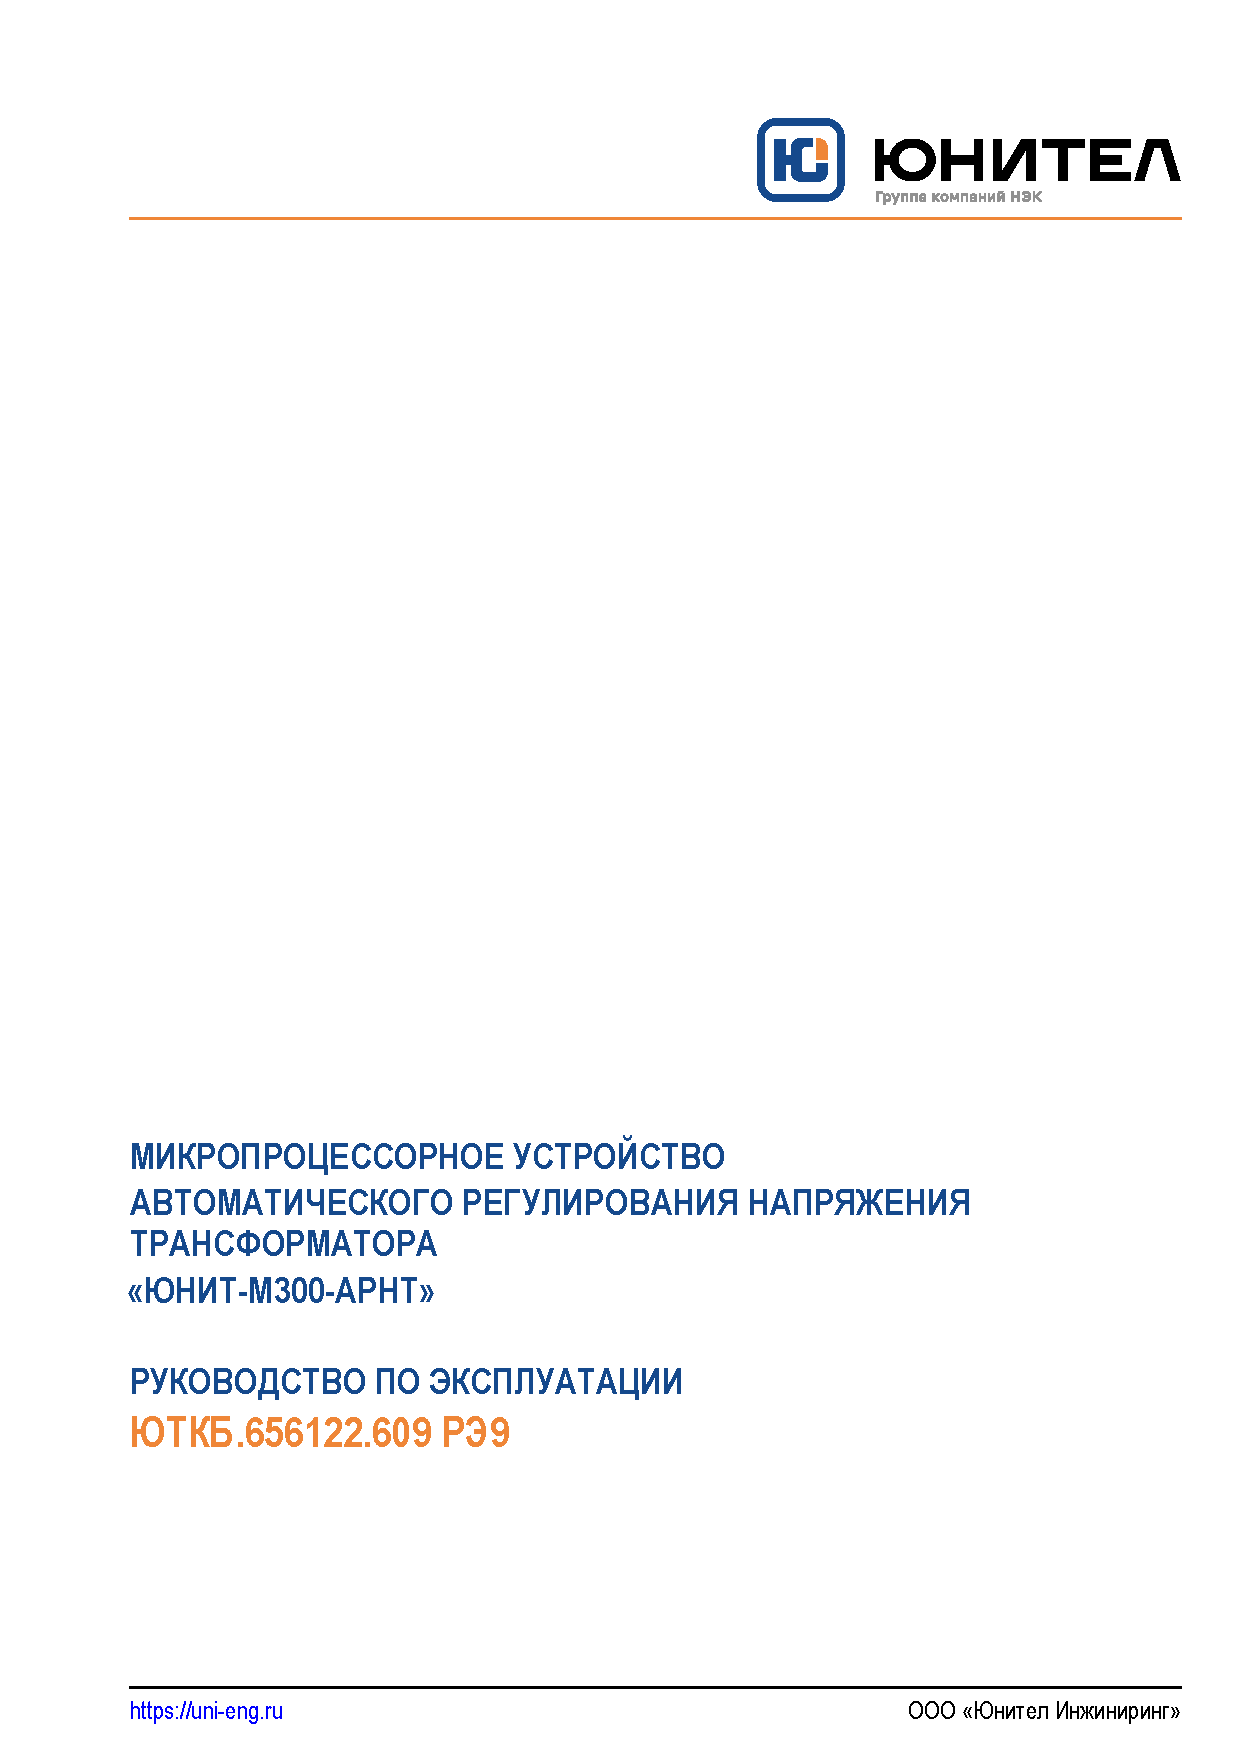
\includepdf[pages={1},width=0.5\textwidth, angle=90]{1.pdf} вставляем и поворачиваем pdf
%\begin{center}
%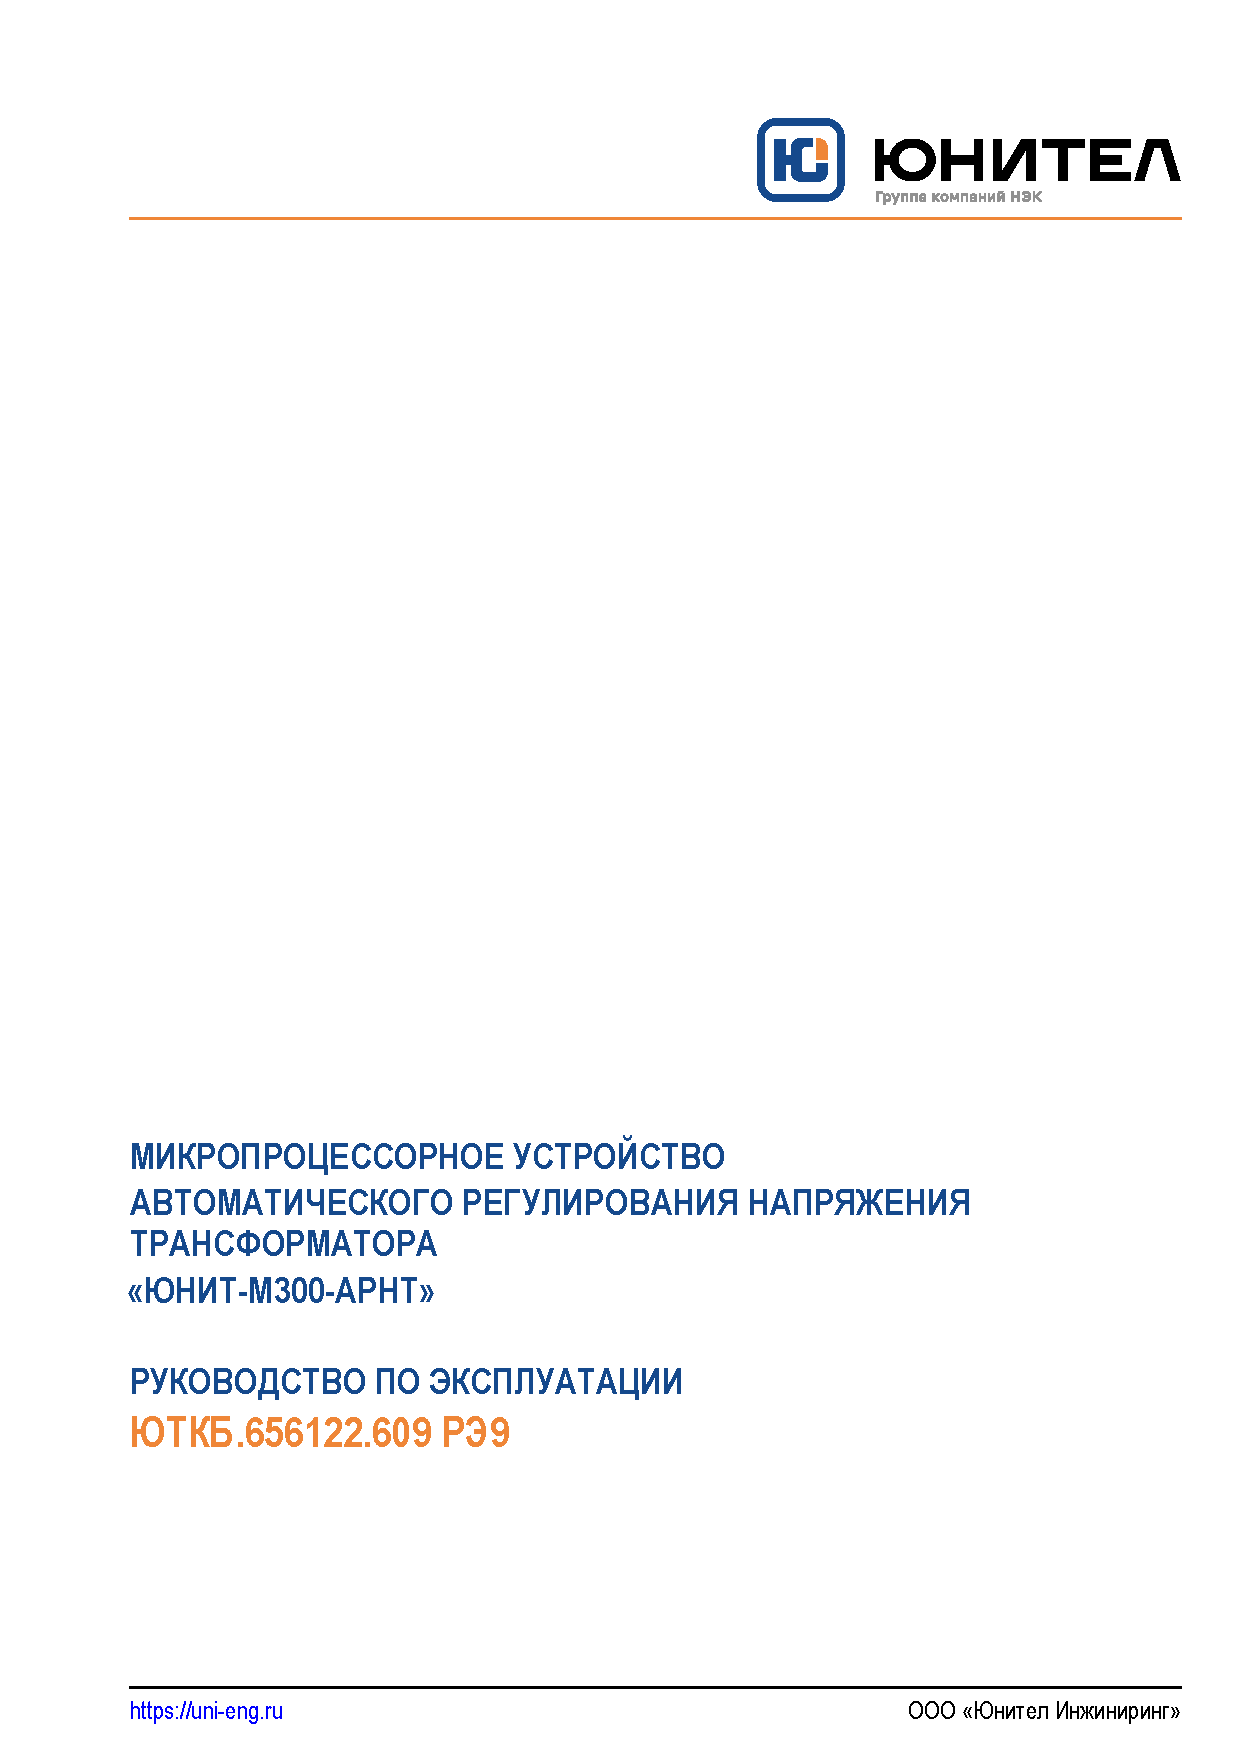
\includegraphics[width=1.4\textwidth]{1.pdf}
%\end{center}

\end{landscape}
\restoregeometry
